\chapter{Structures}

\section{STRUCTURES AND ISOMORPHISMS}

The purpose of this chapter is to describe once and for all a certain number of formative constructions and proofs (cf.~Chapter I, § 1, no. 3 and § 2, no. 2) which arise very frequently in mathematics.

\subsection{ECHELONS}

An echelon construction scheme is a sequence \(c_1, c_2, \ldots, c_m\) of ordered pairs of natural integers (*) \(c_i = (a_i, b_i)\) , satisfying the following conditions:

\begin{enumerate}
\def\labelenumi{(\alph{enumi})}
\item
  If \(b_{i} = 0\) , then \(1 \leqslant a_{i} \leqslant i - 1\) .
\item
  If \(a_i \neq 0\) and \(b_i \neq 0\) , then \(1 \leqslant a_i \leqslant i - 1\) and \(1 \leqslant b_i \leqslant i - 1\) .
\end{enumerate}

These conditions imply that \(c_{1}=(0,b_{1})\) , with \(b_{1}>0\) . If n is the largest of the integers \(b_{i}\) which appear in the pairs \((0,b_{i})\) , then \(c_{1},c_{2},\ldots,c_{m}\) is said to be an echelon construction scheme on n terms.

Given an echelon construction scheme \(\mathbf{S} = (c_{1}, c_{2}, \ldots, c_{m})\) on n terms, and given n terms \(E_{1}, E_{2}, \ldots, E_{n}\) in a theory C which is stronger than the theory of sets, an echelon construction of scheme S on \(E_{1}, \ldots, E_{n}\) is defined to be a sequence \(A_{1}, A_{2}, \ldots, A_{m}\) of m terms in the theory C, defined step by step by the following conditions:

\begin{enumerate}
\def\labelenumi{(\alph{enumi})}
\item
  If \(c_{i} = (0, b_{i})\) , then \(A_{i}\) is the term \(E_{b_{i}}\) .
\item
  If \(c_{i} = (a_{i}, 0)\) , then \(A_{i}\) is the term \(\mathfrak{P}(A_{a_i})\) .
\item
  If \(c_{i} = (a_{i}, b_{i})\) , where \(a_{i} \neq 0\) and \(b_{i} \neq 0\) , then \(A_{i}\) is the term \(A_{a_{i}} \times A_{b_{i}}\) .
\end{enumerate}

The last term \(A_{m}\) of the echelon construction of scheme S on \(E_{1}, \ldots, E_{n}\) is called the echelon of scheme S on the base sets \(E_{1}, \ldots, E_{n}\) ; in the general arguments which follow, it will be denoted by the notation \(S(E_{1}, \ldots, E_{n})\) .

Example. Given two sets E, F, the set \(\mathfrak{P}(\mathfrak{P}(E)) \times \mathfrak{P}(F)\) is an echelon on E, F, with scheme

\[
(0, 1), (0, 2), (1, 0), (3, 0), (2, 0), (4, 5).
\]

It is also the echelon on E, F with scheme

\[
(0, 2), (0, 1), (1, 0), (2, 0), (4, 0), (5, 3).
\]

Distinct schemes may therefore give rise to the same echelon on the same terms.

\subsection{CANONICAL EXTENSIONS OF MAPPINGS}

Let \(S = (c_1, c_2, \ldots, c_m)\) be an echelon construction scheme on \(n\) terms. Let \(E_1, \ldots, E_n, E_1', \ldots, E_n'\) be sets (terms in \(\mathcal{G}\) ) and let \(f_1, \ldots, f_n\) be terms in \(\mathcal{G}\) such that the relations `` \(f_i\) is a mapping of \(E_i\) into \(E_i'\) '' are theorems in \(\mathcal{G}\) for \(1 \leqslant i \leqslant n\) . Let \(A_1, \ldots, A_m\) (resp. \(A_1', \ldots, A_m'\) ) be the echelon construction of scheme S on \(E_1, \ldots, E_n\) (resp. \(E_1', \ldots, E_n'\) ). We define step by step a sequence of \(m\) terms \(g_1, \ldots, g_m\) such that \(g_i\) is a mapping of \(A_i\) into \(A_i'\) (for \(1 \leqslant i \leqslant m\) ) by the following conditions:

\begin{enumerate}
\def\labelenumi{(\alph{enumi})}
\item
  If \(c_{i} = (0, b_{i})\) , so that \(A_{i} = E_{b_{i}}\) and \(A_{i}' = E_{b_{i}}'\) , then \(g_{i}\) is the mapping \(f_{b_{i}}\) .
\item
  If \(c_{i} = (a_{i}, 0)\) , so that \(\mathbf{A}_{i} = \mathfrak{P}(\mathbf{A}_{a_{i}})\) and \(\mathbf{A}_{i}' = \mathfrak{P}(\mathbf{A}_{a_{i}}')\) , then \(g_{i}\) is the canonical extension \(\hat{g}_{a_i}\) of \(g_{a_i}\) to sets of subsets (Chapter II, § 5, no. 1).
\item
  If \(c_{i} = (a_{i}, b_{i})\) , where \(a_{i} \neq 0\) and \(b_{i} \neq 0\) , so that
\end{enumerate}

\[
\mathrm{A} _ {i} = \mathrm{A} _ {a _ {i}} \times \mathrm{A} _ {b _ {i}} \quad \text { and } \quad \mathrm{A} _ {i} ^ {\prime} = \mathrm{A} _ {a _ {i}} ^ {\prime} \times \mathrm{A} _ {b _ {i}} ^ {\prime},
\]

then \(g_{i}\) is the canonical extension \(g_{a_i} \times g_{b_i}\) of \(g_{a_i}\) and \(g_{b_i}\) to \(A_{a_i} \times A_{b_i}\) (Chapter II, § 3, no. 9).

The last term \(g_{m}\) of this sequence is called the canonical extension, with scheme S, of the mappings \(f_{1}, \ldots, f_{n}\) , and will be denoted by \(\langle f_{1}, \ldots, f_{n} \rangle^{S}\) . The following criteria can be verified step by step:

CST1. If \(f_{i}\) is a mapping of \(\mathbf{E}_i\) into \(\mathbf{E}_i'\) , and if \(f_{i}'\) is a mapping of \(\mathbf{E}_i'\) into \(\mathbf{E}_i''\) ( \(1 \leqslant i \leqslant n\) ), then for every echelon construction scheme S on \(n\) terms we have

\[
\langle f _ {1} ^ {\prime} \circ f _ {1}, f _ {2} ^ {\prime} \circ f _ {2}, \dots , f _ {n} ^ {\prime} \circ f _ {n} \rangle^ {\mathrm{S}} = \langle f _ {1} ^ {\prime}, f _ {2} ^ {\prime}, \dots , f _ {n} ^ {\prime} \rangle^ {\mathrm{S}} \circ \langle f _ {1}, f _ {2}, \dots , f _ {n} \rangle^ {\mathrm{S}}.
\]

CST2. If \(f_{i}\) is injective (resp. surjective) for \(1 \leqslant i \leqslant n\) , then \(\langle f_{1}, \ldots, f_{n} \rangle^{S}\) is injective (resp. surjective).

This criterion follows from the corresponding properties of the extension \(\hat{g}\) (Chapter II, § 5, no. 1, Proposition 1) and the extension \(g \times h\) (Chapter II, § 3, no. 9).

CST3. If \(f_{i}\) is a bijection of \(\mathbf{E}_i\) onto \(\mathbf{E}_i'\) , and if \(f_{i}^{-1}\) is the inverse bijection (*), then \(\langle f_1, \ldots, f_n \rangle^{S}\) is a bijection and \(\langle f_1^{-1}, \ldots, f_n^{-1} \rangle^{S}\) is its inverse; in other words,

\[
(\langle f _ {1}, \dots , f _ {n} \rangle^ {\mathrm{S}}) ^ {- 1} = \langle f _ {1} ^ {- 1}, \dots , f _ {n} ^ {- 1} \rangle^ {\mathrm{S}}.
\]

This follows immediately from CST1 and CST2.

\subsection{TRANSPORTABLE RELATIONS}

Let \(\mathfrak{C}\) be a theory which is stronger than the theory of sets, let \(x_{1},\ldots ,x_{n},\) \(s_1,\ldots ,s_p\) be distinct letters which are distinct from the constants of \(\mathfrak{C}\) , and let \(\mathrm{A}_1,\ldots ,\mathrm{A}_m\) be terms in \(\mathfrak{C}\) in which none of the letters \(x_{i}\) \((1\leqslant i\leqslant n)\) and \(s_j\) \((1\leqslant j\leqslant p)\) appears. Let \(\mathrm{S}_1,\ldots ,\mathrm{S}_p\) be echelon construction schemes on \(n + m\) terms. Then the relation \(\mathrm{T}\{x_1,\dots,x_n,s_1,\dots,s_p\}\) :

\[
\begin{array}{c}
\text{``}s_{1} \in S_{1}(x_{1}, \ldots, x_{n}, A_{1}, \ldots, A_{m})
\text{ and }s_{2} \in S_{2}(x_{1}, \ldots, x_{n}, A_{1}, \ldots, A_{m}) \\
\text{and }\ldots\text{ and }s_{p} \in S_{p}(x_{1}, \ldots, x_{n}, A_{1}, \ldots, A_{m})\text{''}
\end{array}
\]

is called a typification of the letters \(s_{1}, \ldots, s_{p}\) .

Let \(\mathbb{R}\{x_1, \ldots, x_n, s_1, \ldots, s_p\}\) be a relation in \(\mathfrak{C}\) which contains certain of the letters \(x_i, s_j\) (and possibly other letters as well). Then \(\mathbb{R}\) is said to be transportable (in \(\mathfrak{C}\) ) with respect to the typification \(\mathbb{T}\) , the \(x_i (1 \leqslant i \leqslant n)\) being considered as principal base sets and the \(A_h (1 \leqslant h \leqslant m)\) as auxiliary base sets, if the following condition is satisfied: let \(y_1, \ldots, y_n, f_1, \ldots, f_n\) be distinct letters which are distinct from the \(x_i (1 \leqslant i \leqslant n)\) , the \(s_j (1 \leqslant j \leqslant p)\) , the constants of \(\mathfrak{C}\) , and all the letters which appear in \(\mathbb{R}\) or in the terms \(A_h (1 \leqslant h \leqslant m)\) , and let \(\operatorname{Id}_h (1 \leqslant h \leqslant m)\) denote the identity mapping of \(A_h\) on to itself. Then the relation

\begin{enumerate}
\def\labelenumi{(\arabic{enumi})}
\tightlist
\item
  ``T \(\{x_{1},\ldots,x_{n},s_{1},\ldots,s_{p}\}\) and ( \(f_{1}\) is a bijection of \(x_{1}\) onto \(y_{1}\) ) and \ldots{} and ( \(f_{n}\) is a bijection of \(x_{n}\) onto \(y_{n}\) )''
\end{enumerate}

implies, in \(\mathfrak{G}\) , the relation

\[
\mathrm{R} \left\{x _ {1}, \dots , x _ {n}, s _ {1}, \dots , s _ {p} \right\} \Longleftrightarrow \mathrm{R} \left\{y _ {1}, \dots , y _ {n}, s _ {1} ^ {\prime}, \dots , s _ {p} ^ {\prime} \right\},\tag{2}
\]

where

\[
s _ {j} ^ {\prime} = \left\langle f _ {1}, \dots , f _ {n}, \operatorname{Id} _ {1}, \dots , \operatorname{Id} _ {m} \right\rangle^ {S_j} (s _ {j}) \quad (1 \leqslant j \leqslant p).\tag{3}
\]

There is an analogous but simpler definition in the case where there is no auxiliary set.

For example, if \(n = p = 2\) and if the typification \(\mathbf{T}\) is ``\(s_1 \in x_1\) and \(s_2 \in x_1\)'', the relation \(s_1 = s_2\) is transportable. On the other hand, the relation \(x_1 = x_2\) is not transportable.

\subsection{SPECIES OF STRUCTURES}

Let \(\mathfrak{G}\) be a theory which is stronger than the theory of sets. A species of structures in \(\mathfrak{G}\) is a text \(\Sigma\) formed of the following assemblies:

\begin{enumerate}
\def\labelenumi{(\arabic{enumi})}
\item
  a certain number of letters \(x_1, \ldots, x_n, s\) , distinct from each other and from the constants of \(\mathfrak{G}\) ; \(x_1, \ldots, x_n\) are called the principal base sets of the species of structures \(\Sigma\) ;
\item
  a certain number of terms \(A_{1}, \ldots, A_{m}\) in G in which none of the letters \(x_{1}, \ldots, x_{n}, s\) appears, and which are called the auxiliary base sets of \(\Sigma\) ; \(\Sigma\) possibly contains no auxiliary base sets (but it must contain at least one principal base set);
\item
  a typification \(\mathrm{T}\{x_1, \ldots, x_n, s\}\) :
\end{enumerate}

\[
s \in \mathrm{S} (x _ {1}, \dots , x _ {n}, \mathrm{A} _ {1}, \dots , \mathrm{A} _ {m}),
\]

where S is an echelon construction scheme on \(n + m\) terms (no. 1); T \(\{x_{1}, \ldots, x_{n}, s\}\) is called the typical characterization of the species of structures \(\Sigma\) ;

\begin{enumerate}
\def\labelenumi{(\arabic{enumi})}
\setcounter{enumi}{3}
\tightlist
\item
  a relation \(R\{x_{1},\ldots,x_{n},s\}\) which is transportable (in C) with respect to the typification T, the \(x_{i}\) being the principal base sets and the \(A_{h}\) the auxiliary base sets (no. 3); R is called the axiom of the species of structures \(\Sigma\) .
\end{enumerate}

The theory \(C_{\Sigma}\) which has the same axiom schemes as C and whose explicit axioms are those of C, together with the axiom ``T and R'', is called the theory of the species of structures \(\Sigma\) . The constants of \(C_{\Sigma}\) are therefore the constants of C and the letters which appear in T or in R.

Let \(\mathfrak{C}'\) be a theory which is stronger than \(\mathfrak{C}\) , and let \(\mathbf{E}_1, \ldots, \mathbf{E}_n\) , U be terms in \(\mathfrak{C}'\) . In the theory \(\mathfrak{C}'\) , U is said to be a structure of species \(\Sigma\) on the principal base sets \(\mathbf{E}_1, \ldots, \mathbf{E}_n\) , with \(\mathbf{A}_1, \ldots, \mathbf{A}_m\) as auxiliary base sets, if the relation

\[
" \mathrm{T} \left\{\mathrm{E} _ {1}, \dots , \mathrm{E} _ {n}, \mathrm{U} \right\} \text { and } \mathrm{R} \left\{\mathrm{E} _ {1}, \dots , \mathrm{E} _ {n}, \mathrm{U} \right\}"
\]

is a theorem in \(\mathfrak{C}'\) . When this is so, then for each theorem \(\mathbf{B}\{x_1, \ldots, x_n, s\}\) in the theory \(\mathfrak{C}_{\Sigma}\) the relation \(\mathbf{B}\{\mathrm{E}_1, \ldots, \mathrm{E}_n, \mathrm{U}\}\) is a theorem in \(\mathfrak{C}'\) (Chapter I, § 2, no. 3). In \(\mathfrak{C}_{\Sigma}\) , the constant \(s\) is called the generic structure of the species \(\Sigma\) .

In the theory \(\mathfrak{G}'\) , the principal base sets \(\mathbf{E}_1, \ldots, \mathbf{E}_n\) are said to be endowed with the structure U. Clearly, U is an element of the set

\[
\mathrm{S} (\mathbf {E} _ {1}, \dots , \mathbf {E} _ {n}, \mathbf {A} _ {1}, \dots , \mathbf {A} _ {m}).
\]

The set of elements V of \(\mathrm{S}(\mathbf{E}_{1},\ldots,\mathbf{E}_{n},\mathbf{A}_{1},\ldots,\mathbf{A}_{m})\) which satisfy the relation \(R\{\mathbf{E}_{1},\ldots,\mathbf{E}_{n},\mathbf{V}\}\) is therefore the set of structures of the species \(\Sigma\) on \(E_{1},\ldots,E_{n}\) (and it may be empty).

Examples

\begin{enumerate}
\def\labelenumi{(\arabic{enumi})}
\tightlist
\item
  Take \(\mathfrak{C}\) to be the theory of sets, and consider the species of structures which has no auxiliary base set, one principal base set A, the typical characterization \(s \in \mathfrak{P}(A \times A)\) , and the axiom
\end{enumerate}

\[
s \circ s = s \quad \text { and } \quad s \cap \overline{s} = \Delta_{\mathbf{A}}
\]

\((\Delta_{\mathbf{A}}\) being the diagonal of \(\mathbf{A} \times \mathbf{A})\) , which is a transportable relation with respect to the typification \(s \in \mathfrak{P}(\mathbf{A} \times \mathbf{A})\) , as is easily verified. It is clear that the theory of this species of structures is just the theory of ordered sets (Chapter III, §1, no. 3); and therefore the species of structure so defined is also called the species of order structures on \(\mathbf{A}\) . In Chapter III we saw many examples of sets endowed with structures of this species.

\begin{enumerate}
\def\labelenumi{(\arabic{enumi})}
\setcounter{enumi}{1}
\item
  Take \(\mathfrak{G}\) to be the theory of sets, and consider the species of structures which has no auxiliary base set, one principal base set A, the typical characterization \(F \in \mathfrak{P}((A \times A) \times A)\) , and as axiom the transportable relation ``F is a functional graph whose domain is \(A \times A\)''. The structures of this species are particular cases of what are called algebraic structures, and the function whose graph is F (a mapping of \(A \times A\) into A) is called the (everywhere defined) internal law of composition of such a structure.
\item
  As before, let \(\mathfrak{C}\) be the theory of sets, and consider the species of structures which has no auxiliary base set, one principal base set A, the typical characterization \(V \in \mathfrak{P}(\mathfrak{P}(A))\) , and as axiom the transportable relation
\end{enumerate}

\[
\begin{array}{l} (\forall \mathrm{V}) ((\mathrm{V} ^ {\prime} \subset \mathrm{V}) \Longrightarrow ((\bigcup_ {\mathrm{X} \in \mathrm{V} ^ {\prime}} \mathrm{X}) \in \mathrm{V})) \\ \text { and } \quad (\forall \mathrm{X}) (\forall \mathrm{Y}) ((\mathrm{X} \in \mathrm{V} \text {   and   } \mathrm{Y} \in \mathrm{V}) \Longrightarrow ((\mathrm{X} \cap \mathrm{Y}) \in \mathrm{V})). \end{array}
\]

This species of structures is called the species of topological structures. A structure of this species is also called a topology, and the relation \(X \in V\) is expressed by saying that X is an open set in the topology V (General Topology, Chapter I, § 1).

* (4) Take \(\mathfrak{G}\) to be the theory of the species of division ring structures, which has (among other things) a constant K as unique (principal) base set. The species of structure of a left vector space over K has K as auxiliary base set, a principal base set E, and as typical characterization the relation

\[
\mathbf {V} \in \mathfrak {P} ((\mathbf {E} \times \mathbf {E}) \times \mathbf {E}) \times \mathfrak {P} ((\mathbf {K} \times \mathbf {E}) \times \mathbf {E})
\]

\((pr_{1}V \text{ being the graph of addition in } E, \text{ and } pr_{2}V \text{ the graph of scalar multiplication}); \text{ we shall not state here the axiom for this species of structures.}\)

\begin{enumerate}
\def\labelenumi{(\arabic{enumi})}
\setcounter{enumi}{4}
\tightlist
\item
  Again let \(\mathfrak{G}\) be the theory of sets; in this theory, the field \(\mathbf{C}\) of complex numbers is a term which contains no letters. The species of structure of a complex analytic manifold of dimension \(n\) has \(\mathbf{C}\) as auxiliary base set, and one principal base set \(V\) . We shall not indicate here the typical characterization or the axiom of this species of structure. *
\end{enumerate}

\minorheading{Remarks}

\begin{enumerate}
\def\labelenumi{(\arabic{enumi})}
\tightlist
\item
  In applications it is often the case (as in Example 4 above) that the echelon \(S(E_1, \ldots, E_n, A_1, \ldots, A_m)\) is a product of echelons
\end{enumerate}

\[
\mathrm{S} _ {1} \left(\mathrm{E} _ {1}, \dots , \mathrm{A} _ {m}\right) \times \dots \times \mathrm{S} _ {p} \left(\mathrm{E} _ {1}, \dots , \mathrm{A} _ {m}\right).
\]

If so, the letter \(s\) in the definition of \(\Sigma\) is often replaced by a `` \(p\) -tuple'' \((s_{1}, \ldots, s_{p})\) (cf.~Chapter II, § 2, no. 1).

Moreover, the axiom of a species of structures \(\Sigma\) is most frequently written as a conjunction of several transportable relations (as in Example 3 above). These relations are called the axioms of the species \(\Sigma\) .

\begin{enumerate}
\def\labelenumi{(\arabic{enumi})}
\setcounter{enumi}{1}
\item
  Names are given to the species of structures most frequently used in mathematics, and to sets endowed with structures of these species. Thus an ordered set (Chapter III, §1) is a set endowed with an order structure (Example 1); * in the later Books of this series, we shall define the notions of group, field, topological space, differentiable manifold, etc., all of which denote sets endowed with certain structures. *
\item
  By abuse of language, in the theory of sets \(\mathfrak{G}\) , the giving of \(n\) distinct letters \(x_{1},\ldots,x_{n}\) (with no typical characterization and no axiom) is considered as a species of structure \(\Sigma_{0}\) , called the structure of a set on the \(n\) principal base sets \(x_{1},\ldots,x_{n}\) .
\end{enumerate}

\subsection{ISOMORPHISMS AND TRANSPORT OF STRUCTURES}

Let \(\Sigma\) be a species of structures in a theory \(\mathfrak{C}\) , on \(n\) principal base sets \(x_{1},\ldots ,x_{n}\) , with \(m\) auxiliary base sets \(\mathbf{A}_1,\dots ,\mathbf{A}_m\) . Let \(\mathbf{S}\) be the echelon construction scheme on \(n + m\) letters which features in the typical characterization of \(\Sigma\) , and let \(\mathbf{R}\) be the axiom of \(\Sigma\) . In a theory \(\mathfrak{C}'\) which is stronger than \(\mathfrak{C}\) , let \(\mathbf{U}\) be a structure of species \(\Sigma\) on sets \(\mathbf{E}_1,\ldots ,\mathbf{E}_n\) (as principal base sets) and let \(\mathbf{U}'\) be a structure of the same species on sets \(\mathbf{E}_1',\ldots ,\mathbf{E}_n'\) . Finally, let \(f_{i}\) (in \(\mathfrak{C}'\) ) be a bijection of \(\mathbf{E}_i\) onto \(\mathbf{E}_i'\) ( \(1 \leqslant i \leqslant n\) ). Then \((f_1, \ldots, f_n)\) is said to be an isomorphism of the sets \(\mathbf{E}_1, \ldots, \mathbf{E}_n\) , endowed with the structure \(\mathbf{U}\) , onto the sets \(\mathbf{E}_1', \ldots, \mathbf{E}_n'\) , endowed with the structure \(\mathbf{U}'\) , if we have (in \(\mathfrak{C}'\) )

\[
\langle f _ {1}, \dots , f _ {n}, \operatorname{Id} _ {1}, \dots , \operatorname{Id} _ {m} \rangle^ {\mathrm{s}} (\mathrm{U}) = \mathrm{U} ^ {\prime}\tag{4}
\]

where \(Id_{h}\) denotes the identity mapping of \(A_{h}\) onto itself ( \(1 \leqslant h \leqslant m\) ). ¶ Let \(f_{i}^{\prime}\) be the inverse of the bijection \(f_{i}\) ( \(1 \leqslant i \leqslant n\) ). It follows immediately from (4) and the criterion CST3 (no. 2) that we have

\[
\langle f _ {1} ^ {\prime}, \dots , f _ {n} ^ {\prime}, \operatorname{Id} _ {1}, \dots , \operatorname{Id} _ {m} \rangle^ {\mathrm{s}} (\mathbf {U} ^ {\prime}) = \mathbf {U}
\]

and consequently that \((f_1', \ldots, f_n')\) is an isomorphism of \(\mathbf{E}_1', \ldots, \mathbf{E}_n'\) , endowed with \(\mathbf{U}'\) , onto \(\mathbf{E}_1, \ldots, \mathbf{E}_n\) , endowed with \(\mathbf{U}\) . The isomorphisms \((f_1, \ldots, f_n)\) and \((f_1', \ldots, f_n')\) are said to be inverses of each other.

\(E_{1}^{\prime}, \ldots, E_{n}^{\prime}\) , endowed with \(U^{\prime}\) , are said to be isomorphic to \(E_{1}, \ldots, E_{n}\) , endowed with U, if there exists an isomorphism of \(E_{1}, \ldots, E_{n}\) onto \(E_{1}^{\prime}, \ldots, E_{n}^{\prime}\) ; in this case the structures U and \(U^{\prime}\) are said to be isomorphic. The above definitions, together with CST1, imply the following criterion:

CST4. Let U, \(U'\) , \(U''\) be three structures of the same species \(\Sigma\) on the principal base sets \(E_{1}, \ldots, E_{n}, E_{1}', \ldots, E_{n}', E_{1}'', \ldots, E_{n}''\) , respectively. Let \(f_{i}\) be a bijection of \(E_{i}\) onto \(E_{i}'\) , and let \(g_{i}\) be a bijection of \(E_{i}'\) onto \(E_{i}''\) ( \(1 \leqslant i \leqslant n\) ). If \((f_{1}, \ldots, f_{n})\) and \((g_{1}, \ldots, g_{n})\) are isomorphisms, then so is \((g_{1} \circ f_{1}, \ldots, g_{n} \circ f_{n})\) .

An isomorphism of \(E_{1}, \ldots, E_{n}\) onto \(E_{1}, \ldots, E_{n}\) (with respect to the same structure) is called an automorphism of \(E_{1}, \ldots, E_{n}\) . The composition of two automorphisms of \(E_{1}, \ldots, E_{n}\) is an automorphism, and so is the inverse of an automorphism, * so that the automorphisms of \(E_{1}, \ldots, E_{n}\) form a group. *

Remark. By abuse of language, if \(f_{i}\) is any bijection of \(\mathbf{E}_i\) onto \(\mathbf{E}_i'\) ( \(1 \leqslant i \leqslant n\) ), \((f_1, \ldots, f_n)\) is said to be an isomorphism of \(\mathbf{E}_1, \ldots, \mathbf{E}_n\) onto \(\mathbf{E}_1', \ldots, \mathbf{E}_n'\) with respect to the species of structure of a set (no. 4, Remark 3).

CST5. In a theory \(\mathfrak{G}'\) which is stronger than \(\mathfrak{G}\) , let U be a structure of species \(\Sigma\) on \(\mathbf{E}_1, \ldots, \mathbf{E}_n\) , and let \(f_i\) be a bijection of \(\mathbf{E}_i\) onto a set \(\mathbf{E}_i'\) ( \(1 \leqslant i \leqslant n\) ). Then there exists a unique structure of species \(\Sigma\) on \(\mathbf{E}_1', \ldots, \mathbf{E}_n'\) such that \((f_1, \ldots, f_n)\) is an isomorphism of \(\mathbf{E}_1, \ldots, \mathbf{E}_n\) onto \(\mathbf{E}_1', \ldots, \mathbf{E}_n'\) .

For this structure, if it exists, can only be the term \(U'\) defined by the relation (4); it remains to be verified that this term is indeed a structure of species \(\Sigma\) , i.e., that the relation \(R\{E_{1}', \ldots, E_{n}', U'\}\) is true in \(C'\) . But this follows from the fact that \(R\{x_{1}, \ldots, x_{n}, s\}\) is transportable, for

\(R\{E_{1}^{\prime},\ldots,E_{n}^{\prime},U^{\prime}\}\) is equivalent in \(C'\) to the relation \(R\{E_{1},\ldots,E_{n},U\}\) (no. 3), which is true in \(C'\) by hypothesis.

The structure \(U'\) is said to be obtained by transporting the structure U to the sets \(E_{1}^{\prime}, \ldots, E_{n}^{\prime}\) by means of the bijective mappings \(f_{1}, \ldots, f_{n}\) . Thus two structures of the same species are isomorphic if and only if each is obtained from the other by transport of structure.

It may happen that any two structures of species \(\Sigma\) are necessarily isomorphic; the species of structure \(\Sigma\) is then said be univalent. * This is the case for the structure of an infinite cyclic group (isomorphic to \(\mathbf{Z}\) ), the structure of a prime field of characteristic zero (isomorphic to \(\mathbf{Q}\) ), the structure of a complete Archimedean ordered field (isomorphic to \(\mathbf{R}\) ), the structure of an algebraically closed, connected, locally compact topological field (isomorphic to \(\mathbf{C}\) ), and of the structure of a non-commutative, connected, locally compact topological division ring (isomorphic to \(\mathbf{H}\) , the division ring of quaternions). For some of these species of structure, for example that of a prime field of characteristic zero, or that of a complete Archimedean ordered field, there is not even any automorphism other than the identity mapping; but there do exist such automorphisms for the other examples given above (for example, the symmetry \(x \to -x\) in \(\mathbf{Z}\) ). *

It will be observed that the above species of structure are essentially those which are the basis of classical mathematics. On the other hand, * the species of group structures, the species of structures of an ordered set, and the species of topological structures, are not univalent. *

\subsection{DEDUCTION OF STRUCTURES}

Let \(\Sigma\) be a species of structures in a theory \(\mathfrak{G}\) , on \(n\) principal base sets \(x_{1},\ldots ,x_{n}\) , with \(m\) auxiliary base sets \(\mathrm{A}_1,\dots ,\mathrm{A}_m\) . Let \(s\) be the generic structure of \(\Sigma\) , and let \(\mathbf{T}\) be an echelon construction scheme on \(n + m\) terms. A term \(\mathrm{V}\{x_1,\dots,x_n,s\}\) which contains no letter other than the constants of \(\mathfrak{G}_{\Sigma}\) is said to be intrinsic for \(s\) , of type \(\mathrm{T}(x_1,\dots,x_n,\mathrm{A}_1,\dots,\mathrm{A}_m)\) , if it satisfies the following conditions:

\begin{enumerate}
\def\labelenumi{(\arabic{enumi})}
\item
  the relation \(\mathbf{V}\{x_1, \ldots, x_n, s\} \in \mathbf{T}(x_1, \ldots, x_n, A_1, \ldots, A_m)\) is a theorem in \(\mathfrak{G}_{\Sigma}\) ;
\item
  let \(\mathfrak{G}_{\Sigma}^{\prime}\) be the theory obtained by adjoining to the axioms of \(\mathfrak{G}_{\Sigma}\) the axioms '' \(f_{i}\) is a bijection of \(x_{i}\) onto \(y_{i}''\) ( \(1 \leqslant i \leqslant n\) ) (where the letters \(y_{i}\) and \(f_{i}\) are distinct from each other and from the constants of \(\mathfrak{G}_{\Sigma}\) , for \(1 \leqslant i \leqslant n\) ); if \(s'\) is the structure obtained by transporting \(s\) by means of \((f_{1}, \ldots, f_{n})\) (no. 5), then
\end{enumerate}

\[
\mathrm{V} \left\{y _ {1}, \dots , y _ {n}, s ^ {\prime} \right\} = \langle f _ {1}, \dots , f _ {n}, \operatorname{Id} _ {1}, \dots , \operatorname{Id} _ {m} \rangle^ {\mathrm{T}} (\mathrm{V} \left\{x _ {1}, \dots , x _ {n}, s \right\})
\]

is a theorem in \(\mathfrak{C}_{\Sigma}^{\prime}\) .

Most of the terms which one is led to define in the theory of a species of structures are intrinsic terms.

Let \(\Theta\) be another species of structures in the theory \(\mathfrak{G}\) , on \(r\) principal base sets \(u_{1},\ldots,u_{r}\) , with \(p\) auxiliary base sets \(\mathrm{B}_{1},\ldots,\mathrm{B}_{p}\) , and let \(t\in\mathrm{T}(u_{1},\ldots,u_{r},\mathrm{B}_{1},\ldots,\mathrm{B}_{p})\) be the typical characterization of \(\Theta\) (no. 4). Then a system of \(r+1\) terms \(\mathrm{P},\mathrm{U}_{1},\ldots,\mathrm{U}_{r}\) , intrinsic for \(s\) , and such that \(\mathrm{P}\) is a structure of species \(\Theta\) on \(\mathrm{U}_{1},\ldots,\mathrm{U}_{r}\) , in the theory \(\mathfrak{G}_{\Sigma}\) , is called a procedure of deduction of a structure of species \(\Theta\) from a structure of species \(\Sigma\) . By abuse of language, the term \(\mathrm{P}\) alone is often called a procedure of deduction.

Let \(\mathfrak{G}'\) be a theory stronger than \(\mathfrak{G}\) . If \(\mathcal{G}\) is a structure in \(\mathfrak{G}'\) of species \(\Sigma\) on \(\mathrm{E}_1, \ldots, \mathrm{E}_n\) , then \(\mathrm{P}\{\mathrm{E}_1, \ldots, \mathrm{E}_n, \mathcal{S}\}\) is a structure of species \(\Theta\) on the \(r\) sets \(\mathrm{F}_j = \mathrm{U}_j\{\mathrm{E}_1, \ldots, \mathrm{E}_n, \mathcal{S}\}(1 \leqslant j \leqslant r)\) , said to be deduced from \(\mathcal{S}\) by the procedure P, or subordinate to \(\mathcal{G}\) . The hypothesis that the terms P, \(\mathrm{U}_1, \ldots, \mathrm{U}_r\) are intrinsic for \(s\) moreover implies the following criterion:

CST6. Let \((g_{1}, \ldots, g_{n})\) be an isomorphism of \(E_{1}, \ldots, E_{n}\) , endowed with a structure S of species \(\Sigma\) , onto \(E_{1}^{\prime}, \ldots, E_{n}^{\prime}\) , endowed with a structure \(S^{\prime}\) of the same species. If \(U_{j}\) is of type \(\mathfrak{P}(T_{j})\) , put

\[
h _ {j} = \left\langle g _ {1}, \dots , g _ {n}, \operatorname{Id} _ {1}, \dots , \operatorname{Id} _ {m} \right\rangle^ {\mathrm{T}_j} \quad (1 \leqslant j \leqslant r),
\]

and let \(\mathbf{F}_j' = \mathbf{U}_j\{\mathbf{E}_1', \ldots, \mathbf{E}_n', \mathcal{S}'\} (1 \leqslant j \leqslant r)\) . Then \((h_1, \ldots, h_r)\) is an isomorphism of \(\mathbf{F}_1, \ldots, \mathbf{F}_r\) onto \(\mathbf{F}_1', \ldots, \mathbf{F}_r'\) when these systems of sets are endowed with the structures of species \(\Theta\) deduced from \(\mathcal{S}\) and \(\mathcal{S}'\) respectively by the procedure P.

It is clear that the terms \(x_{1}, \ldots, x_{n}\) are intrinsic for \(s\) . In many cases, the terms \(U_{1}, \ldots, U_{r}\) are certain of the letters \(x_{1}, \ldots, x_{n}\) ; the structure of species \(\Theta\) deduced from \(s\) by the procedure \(P\) is then said to be a structure underlying \(s\) .

\minorheading{Examples}

* (1) The species of topological group structures has a single principal base set A, no auxiliary base set, and the corresponding generic structure is a pair \((s_1, s_2)\) ( \(s_1\) being the graph of the law of composition on A, and \(s_2\) the set of open sets in the topology of A; cf.~General Topology, Chapter III, § 1). Each of the terms \(s_1\) , \(s_2\) is a procedure of deduction and provides respectively the group structure and the topology underlying the topological group structure \((s_1, s_2)\) .

Likewise, from a vector space structure can be deduced an underlying commutative group structure. From a ring structure can be deduced an underlying commutative group structure and a (multiplicative) semigroup structure. From the structure of a differentiable manifold can be deduced an underlying topology, etc.

\begin{enumerate}
\def\labelenumi{(\arabic{enumi})}
\setcounter{enumi}{1}
\tightlist
\item
  The species of vector space structures over C (resp. R) has a principal base set E, an auxiliary base set equal to C (resp. R), and typical characterization
\end{enumerate}

\[
s _ {1} \in \mathfrak {P} ((\mathbf {E} \times \mathbf {E}) \times \mathbf {E}) \quad \text { and } \quad s _ {2} \in \mathfrak {P} ((\mathbf {C} \times \mathbf {E}) \times \mathbf {E})
\]

\[
(\text { resp. } \quad s _ {1} \in \mathfrak {P} ((E \times E) \times E) \quad \text { and } \quad s _ {2} \in \mathfrak {P} ((R \times E) \times E)).
\]

The pair \((s_{1}, s_{2} \cap ((\mathbf{R} \times \mathbf{E}) \times \mathbf{E}))\) is a procedure of deduction of a vector space structure over R from a vector space structure over C (``restriction of the field of scalars to R''). *

\begin{enumerate}
\def\labelenumi{(\arabic{enumi})}
\setcounter{enumi}{2}
\tightlist
\item
  Suppose that \(\Theta\) has the same (principal and auxiliary) base sets as \(\Sigma\) , and the same typical characterization. If, moreover, the axiom of \(\Sigma\) implies (in \(\mathfrak{C}\) ) the axiom of \(\Theta\) , it is clear that the term \(s\) is a procedure of deduction of a structure of species \(\Theta\) from a structure of species \(\Sigma\) . \(\Theta\) is then said to be poorer than \(\Sigma\) , and \(\Sigma\) is richer than \(\Theta\) . Every structure of species \(\Sigma\) , in a theory \(\mathfrak{C}'\) which is stronger than \(\mathfrak{C}\) , is then also a structure of species \(\Theta\) . For example, the species of structures of totally ordered sets (obtained by taking as axiom the conjunction of the
\end{enumerate}

axiom of order structures (no. 4, Example 1) and the relation \(s \cup \overline{s} = A \times A\) ) is richer than the species of order structures. *The species of commutative group structures is richer than the species of group structures. The species of compact topological space structures is richer than the species of topological structures, etc. *

* (4) When each of \(\Sigma\) and \(\Theta\) is the species of group structures (resp. ring structures), there is defined in algebra a procedure of deduction which associates with each group structure (resp. ring structure) the group structure (resp. ring structure) on its centre. When \(\Sigma\) is the species of vector space structures over a field K, and when \(\Theta\) is the species of algebraic structures over K, there are defined procedures of deduction which associate with every vector space over K its tensor algebra or its exterior algebra. We shall meet many other examples later in this series. *

Remark. When P is a ``q-tuple'' \((P_{1}, \ldots, P_{q})\) , it is also said that the terms \(P_{1}, \ldots, P_{q}\) constitute a procedure of deduction of a structure of species \(\Theta\) from a structure of species \(\Sigma\) .

\subsection{EQUIVALENT SPECIES OF STRUCTURES}

Let \(\Sigma\) and \(\Theta\) be two species of structures, in the same theory \(\mathfrak{C}\) , having the same principal base sets \(x_{1},\ldots ,x_{n}\) . Let \(s,t\) be the generic structures of the species \(\Sigma,\Theta\) respectively. Suppose that the following conditions are satisfied:

\begin{enumerate}
\def\labelenumi{(\arabic{enumi})}
\item
  We have a procedure of deduction \(\mathbf{P}\{x_1, \ldots, x_n, s\}\) of a structure of species \(\Theta\) on \(x_1, \ldots, x_n\) from a structure of species \(\Sigma\) on \(x_1, \ldots, x_n\) .
\item
  We have a procedure of deduction \(\mathbb{Q}\{x_1, \ldots, x_n, t\}\) of a structure of species \(\Sigma\) on \(x_1, \ldots, x_n\) from a structure of species \(\Theta\) on \(x_1, \ldots, x_n\) .
\item
  The relation \(\mathbf{Q}\{x_1, \ldots, x_n, \mathbf{P}\{x_1, \ldots, x_n, s\}\} = s\) is a theorem in \(\mathfrak{G}_{\Sigma}\) , and the relation \(\mathbf{P}\{x_1, \ldots, x_n, \mathbf{Q}\{x_1, \ldots, x_n, t\}\} = t\) is a theorem in \(\mathfrak{G}_{\Theta}\) .
\end{enumerate}

The species of structures \(\Sigma\) and \(\Theta\) are then said to be equivalent by means of the procedures of deduction P and Q. In this case, for every theorem B \(\{x_1, \ldots, x_n, s\}\) in the theory \(\mathfrak{G}_{\Sigma}\) , the relation B \(\{x_1, \ldots, x_n, Q\}\) is a theorem in \(\mathfrak{G}_{\Theta}\) ; and conversely, for every theorem C \(\{x_1, \ldots, x_n, t\}\) in the theory \(\mathfrak{G}_{\Theta}\) , the relation C \(\{x_1, \ldots, x_n, P\}\) is a theorem in \(\mathfrak{G}_{\Sigma}\) .

If U is a structure of species \(\Sigma\) , the structure deduced from U by the procedure P is said to be equivalent to U. Criterion CST6 implies the following :

CST7. Let \(\mathcal{S},\mathcal{S}'\) be two structures of species \(\Sigma\) on the principal base sets \((\mathbf{E}_1,\ldots ,\mathbf{E}_n),(\mathbf{E}_1',\ldots ,\mathbf{E}_n')\) , respectively. Let \(\mathcal{S}_0,\mathcal{S}_0'\) be structures of species \(\Theta\) which are equivalent respectively to \(\mathcal{S}\) and \(\mathcal{S}'\) . In order that \((g_1,\dots,g_n)\) should be an isomorphism with respect to the structures \(\mathcal{S}_0\) and \(\mathcal{S}_0'\) , it is necessary and sufficient that \((g_1,\dots,g_n)\) should be an isomorphism with respect to the structures \(\mathcal{S}\) and \(\mathcal{S}'\) .

In practice, we make no distinction between the theories \(\mathfrak{G}_{\Sigma}\) and \(\mathfrak{G}_{\Theta}\) of two equivalent species of structures.

\minorheading{Examples}

* (1) Let \(\Sigma\) be the species of commutative group structures; \(\Sigma\) has a single (principal) base set A, and its generic structure consists of a single letter F; the typical characterization of \(\Sigma\) is \(F \in \mathfrak{P}((A \times A) \times A)\) , and we denote the axiom of \(\Sigma\) by R \{A, F\}. This axiom implies in particular that F is the graph of a function (the ``law of composition'' of the group; cf.~no. 4, Example 2). In the theory \(\mathfrak{G}_{\Sigma}\) (where \(\mathfrak{G}\) denotes the theory of sets) we define a term M\{A, F\} which is a functional graph in \(\mathfrak{P}((Z \times A) \times A)\) and satisfies the following relation B\{M, A, F\}:

\((\forall x)(\forall y)(\forall n)((x \in A \text{ and } y \in A \text{ and } n \in \mathbf{Z})\)

\[
\Longrightarrow (\mathbf {M} (n, \mathrm{F} (x, y)) = \mathrm{F} (\mathbf {M} (n, x), \mathrm{M} (n, y))))
\]

and \((\forall x)(\forall m)(\forall n)((x\in A\) and \(m\in \mathbf{Z}\) and \(n\in \mathbf{Z})\)

\[
\Rightarrow (\mathrm{M} (m + n, x) = \mathrm{F} (\mathrm{M} (m, x), \mathrm{M} (n, x))))
\]

and \((\forall x)(\forall m)(\forall n)((x\in A\) and \(m\in \mathbf{Z}\) and \(n\in \mathbf{Z})\)

\[
\Longrightarrow (\mathbf {M} (m, \mathbf {M} (n, x)) = \mathbf {M} (m n, x)))
\]

and

\[
(\forall x) ((x \in A) \Longrightarrow (M (1, x) = x)).
\]

(``multiplication of an element of A by an integer'').

Consider the species \(\Theta\) of \(\mathbf{Z}\) -module structures, which has a single principal base set A, with \(\mathbf{Z}\) as auxiliary set, and whose generic structure contains two letters G, L, with the typical characterization

\[
\mathbf {G} \in \mathfrak {P} ((\mathbf {A} \times \mathbf {A}) \times \mathbf {A}) \quad \text { and } \quad \mathbf {L} \in \mathfrak {P} ((\mathbf {Z} \times \mathbf {A}) \times \mathbf {A})
\]

and the axiom

\[
\text{``}R\{A,G\}\text{ and }(L\text{ is a functional graph})\text{ and }B\{L,A,G\}\text{''.}
\]

It is immediately verified that the terms F, M constitute a procedure of deduction of a structure of species \(\Theta\) from a structure of species \(\Sigma\) , and that the term G is a procedure of deduction of a structure of species \(\Sigma\) from a structure of species \(\Theta\) . Furthermore, the condition (3) above is trivially satisfied. We may therefore say that the species of commutative group structures and the species of Z-module structures are equivalent.

\begin{enumerate}
\def\labelenumi{(\arabic{enumi})}
\setcounter{enumi}{1}
\tightlist
\item
  Let \(\Sigma\) be the species of topological structures (no. 4, Example 3), let A be the (principal) base set, and let V be the generic structure of \(\Sigma\) . Consider the relation
\end{enumerate}

\[
x \in A \text {   and   } X \subset A \text {   and   } (\forall U) ((U \in V \text {   and   } x \in U) \Longrightarrow (X \cap U \neq \emptyset)).
\]

This relation has a graph \(P \subset \mathfrak{P}(A) \times A\) with respect to the pair \((X, x)\) ; \(P\{A, V\}\) is a term called ``the set of all pairs \((X, x)\) such that x lies in the closure of X with respect to the topology V''. We can then prove (cf.~General Topology, Chapter I, §1) that the following relations are theorems in \(G_{\Sigma}\) :

\[
\begin{array}{c} \mathrm{P} (\phi) = \phi , \\ (\forall \mathrm{Y}) ((\mathrm{Y} \subset \mathrm{A}) \Longrightarrow (\mathrm{Y} \subset \mathrm{P} (\mathrm{Y}))), \\ (\forall \mathrm{Y}) ((\mathrm{Y} \subset \mathrm{A}) \Longrightarrow (\mathrm{P} (\mathrm{P} (\mathrm{Y})) = \mathrm{P} (\mathrm{Y}))), \\ (\forall \mathrm{Y}) (\forall \mathrm{Z}) ((\mathrm{Y} \subset \mathrm{A} \text {and} \mathrm{Z} \subset \mathrm{A}) \Longrightarrow (\mathrm{P} (\mathrm{Y} \cup \mathrm{Z}) = \mathrm{P} (\mathrm{Y}) \cup \mathrm{P} (\mathrm{Z}))). \end{array}
\]

Consider the species of structures \(\Theta\) , having a single (principal) base set A, whose generic structure consists of a single letter W, which has as typical characterization \(W \in \mathfrak{P}(\mathfrak{P}(A) \times A)\) and as axiom

\[
\begin{array}{c} \mathrm{W} (\emptyset) = \emptyset \quad \text {and} \quad (\forall \mathrm{Y}) ((\mathrm{Y} \subset \mathrm{A}) \Longrightarrow (\mathrm{Y} \subset \mathrm{W} (\mathrm{Y}))) \\ \text {and} \quad (\forall \mathrm{Y}) ((\mathrm{Y} \subset \mathrm{A}) \Longrightarrow (\mathrm{W} (\mathrm{W} (\mathrm{Y})) = \mathrm{W} (\mathrm{Y}))) \\ \text {and} \quad (\forall \mathrm{Y}) (\forall \mathrm{Z}) ((\mathrm{Y} \subset \mathrm{A} \quad \text {and} \quad \mathrm{Z} \subset \mathrm{A}) \Longrightarrow (\mathrm{W} (\mathrm{Y} \cup \mathrm{Z}) = \mathrm{W} (\mathrm{Y}) \cup \mathrm{W} (\mathrm{Z}))). \end{array}
\]

Consider also the relation

\[
\mathrm{U} \subset \mathrm{A} \quad \text { and } \quad (\forall x) ((x \in \mathrm{U}) \Longrightarrow x \notin \mathrm{W} (\mathrm{A} - \mathrm{U})).
\]

The set of all \(U \in \mathfrak{P}(A)\) which satisfy this relation is a subset \(Q\{A, W\}\) of \(\mathfrak{P}(A)\) . We can then prove (General Topology, Chapter I, §1, Exercise 10) that the following relations are theorems in \(G_{\Theta}\) :

\[
\begin{array}{c} \mathrm{A} \in \mathrm{Q}, \\ (\forall \mathrm{M}) ((\mathrm{M} \subset \mathrm{Q}) \Longrightarrow \left(\left(\bigcup_ {\mathrm{X} \in \mathrm{M}} \mathrm{X}\right) \in \mathrm{Q}\right), \end{array}
\]

\[
(\forall \mathrm{X}) (\forall \mathrm{Y}) ((\mathrm{X} \in \mathrm{Q} \text {   and   } \mathrm{Y} \in \mathrm{Q}) \Longrightarrow ((\mathrm{X} \cap \mathrm{Y}) \in \mathrm{Q})).
\]

Thus the terms \(P\{A,V\}\) and \(Q\{A,W\}\) satisfy conditions (1) and (2) above, and it is easily seen that they also satisfy condition (3). The species of structures \(\Sigma\) and \(\Theta\) are therefore equivalent, and we therefore consider every structure of species \(\Theta\) as a topology, namely that which corresponds to it under the procedure of deduction \(Q\{A,W\}\). *

\section{MORPHISMS AND DERIVED STRUCTURES}

\subsection{MORPHISMS}

In this section and the next we shall assume for the sake of simplicity that the species of structures under consideration has only one base set (which is therefore a principal base set). The reader will have no difficulty in extending the definitions and results to the general case.

Let \(\Sigma\) be a species of structures in a theory \(\mathcal{C}\) which is stronger than the theory of sets, and let \(x, y, s, t\) be four distinct letters which are different from the constants of \(\mathcal{C}\) . We recall that the notation \(\mathcal{F}(x, y)\) denotes the set of mappings of \(x\) into \(y\) (Chapter II, § 5, no. 2). Suppose that we are given a term \(\sigma\{x, y, s, t\}\) in \(\mathcal{C}\) which satisfies the following conditions:

(MO \(_{I}\) ) The relation `` \(s\) is a structure of species \(\Sigma\) on \(x\) , and \(t\) is a structure of species \(\Sigma\) on \(y\) '' implies, in \(\mathfrak{C}\), the relation \(\sigma\{x,y,s,t\} \subset \mathcal{F}(x,y)\) .

\((\mathrm{MO}_{\mathrm{II}})\) If, in a theory \(\mathfrak{C}'\) stronger than \(\mathfrak{C}\) , we have three sets \(\mathbf{E}\) , \(\mathbf{E}'\) , \(\mathbf{E}''\) endowed respectively with structures \(\mathscr{S}\) , \(\mathscr{S}'\) , \(\mathscr{S}''\) of species \(\Sigma\) , then the relations \(f \in \sigma \{ \mathbf{E}, \mathbf{E}', \mathscr{S}, \mathscr{S}' \}\) and \(g \in \sigma \{ \mathbf{E}', \mathbf{E}'', \mathscr{S}', \mathscr{S}'' \}\) imply the relation

\[
g \circ f \in \sigma \left\{\mathrm{E}, \mathrm{E} ^ {\prime \prime}, \mathscr {S}, \mathscr {S} ^ {\prime \prime} \right\}.
\]

\((\mathrm{MO}_{\mathrm{III}})\) If, in a theory \(\mathfrak{C}'\) stronger than \(\mathfrak{C}\) , we have two sets \(\mathbf{E}\) , \(\mathbf{E}'\) endowed respectively with structures \(\mathcal{S}\) , \(\mathcal{S}'\) of species \(\Sigma\) , then a bijection \(f\) of \(\mathbf{E}\) onto \(\mathbf{E}'\) is an isomorphism if and only if \(f \in \sigma \left\{\mathbf{E}, \mathbf{E}', \mathcal{S}, \mathcal{S}'\right\}\) and \(f^{-1} \in \sigma \left\{\mathbf{E}', \mathbf{E}, \mathcal{S}', \mathcal{S}\right\}\) .

If \(\Sigma\) and \(\sigma\) are given, the relation \(f \in \sigma\{x, y, s, t\}\) is expressed by saying that \(f\) is a morphism (or a \(\sigma\) -morphism) of \(x\) , endowed with \(s\) , into \(y\) , endowed with \(t\) . If (in a theory \(\mathfrak{G}'\) stronger than \(\mathfrak{G}\) ) \(\mathbf{E}\) and \(\mathbf{E}'\) are two sets endowed with structures \(\mathcal{S}, \mathcal{S}'\) of species \(\Sigma\) , then the term \(\sigma\{\mathbf{E}, \mathbf{E}', \mathcal{S}, \mathcal{S}'\}\) is the set of \(\sigma\) -morphisms of \(\mathbf{E}\) into \(\mathbf{E}'\) .

Examples

\begin{enumerate}
\def\labelenumi{(\arabic{enumi})}
\item
  Take \(\Sigma\) to be the species of order structures and let \(\sigma\{x, y, s, t\}\) denote the set of all mappings \(f\) of \(x\) into \(y\) such that the relation \((u, v) \in s\) implies \((f(u), f(v)) \in t\) . With the notation of Chapter III, § 1, this means that \(u \leqslant v\) implies \(f(u) \leqslant f(v)\) , i.e., that \(f\) is increasing. The verification of axioms \((\mathrm{MO}_{\mathbf{I}}), (\mathrm{MO}_{\mathbf{II}})\) , and \((\mathrm{MO}_{\mathbf{III}})\) is obvious.
\item
  Take \(\Sigma\) to be a species of algebraic structures which has a single (internal) law of composition, everywhere defined (§1, no. 4, Example 2). Let A, A' be two sets endowed with structures of species \(\Sigma\) , and let \(p, p'\) be the composition laws of these two structures. Consider the mappings \(f\) of A into A' such that \(p'(f(x), f(y)) = f(p(x, y))\) for all \(x \in A\) and all \(y \in A\) . These mappings satisfy (MO \(_{I}\) ), (MO \(_{II}\) ), and (MO \(_{III}\) ), and are called homomorphisms of A into A'.
\item
  Take \(\Sigma\) to be the species of topological structures (§1, no. 4, Example 3). Let A, A' be two sets endowed with topologies V, V', respectively. Consider the mappings \(f\) of A into A' such that the
\end{enumerate}

relation \(\mathbf{X}' \in \mathbf{V}'\) implies \(\overline{f}^{1}(\mathbf{X}') \in \mathbf{V}\) (in other words, such that the inverse image of every open set in the topology \(\mathbf{V}'\) is an open set in the topology \(\mathbf{V}\) ). These mappings, which satisfy \((\mathrm{MO}_{\mathbf{I}})\) , \((\mathrm{MO}_{\mathbf{II}})\) , and \((\mathrm{MO}_{\mathbf{III}})\) , are the continuous mappings of \(\mathbf{A}\) into \(\mathbf{A}'\) (with respect to the topologies \(\mathbf{V}\) and \(\mathbf{V}'\) ) (cf.~General Topology, Chapter I, § 2).

Remark. For given species of structures \(\Sigma\) we may have occasion to define various terms \(\sigma \{x, y, s, t\}\) which satisfy the conditions \((\mathrm{MO}_{\mathbf{I}})\) , \((\mathrm{MO}_{\mathbf{II}})\) , and \((\mathrm{MO}_{\mathbf{III}})\) . For example, if \(\Sigma\) is the species of topological structures, with the notation of Example 3 above, a mapping \(f\) of A into \(\mathbf{A}'\) is said to be open if the relation \(\mathbf{X} \in \mathbf{V}\) implies \(f(\mathbf{X}) \in \mathbf{V}'\) (in other words, if the image under \(f\) of every open set is an open set). It is easily checked that the open mappings also satisfy conditions \((\mathrm{MO}_{\mathbf{I}})\) , \((\mathrm{MO}_{\mathbf{II}})\) , and \((\mathrm{MO}_{\mathbf{III}})\) for the species \(\Sigma\) . * Moreover, it can be shown that a continuous mapping is not necessarily open, and that an open mapping is not necessarily continuous. * A given species of structures therefore does not imply a well-defined notion of morphisms.

\pandocbounded{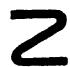
\includegraphics[keepaspectratio]{images/part002_a17f5ac5846160dabe35edfd7ae1b1f71cd54f2b9ab149a24f189ab7736ff1b5.jpg}}

Where order structures, algebraic structures, and topological structures are concerned, it is always to be understood that the morphisms are those which have been defined in the Examples above, unless the contrary is expressly stated.

The condition \((MO_{III})\) and the characterization of bijections (Chapter II, § 3, no. 8, Corollary to Proposition 8) imply the following criterion :

CST8. Let E, E' be two sets, each endowed with a structure of species Σ. Let f be a σ-morphism of E into E' and let g be a σ-morphism of E' into E. If g∘f is the identity mapping of E onto itself, and if f∘g is the identity mapping of E' onto itself, then f is an isomorphism of E onto E', and g is the inverse isomorphism.

\pandocbounded{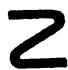
\includegraphics[keepaspectratio]{images/part002_4a2c9e6ca2e0232c08246aaeec85214d3ec9d06a429c17d5fe3c6f33ea15bbf4.jpg}}

It should be noted that a bijection of E onto E' may be a σ-morphism without the inverse bijection necessarily being a σ-morphism. * For example, a bijective mapping of a topological space A onto a topological space A' can be continuous without the inverse bijection being continuous (General Topology, Chapter I, § 2, no. 1, Remark 1). *

Remark. When a species of structures \(\Sigma\) has several principal base sets \(x_{1},\ldots ,x_{n}\) , and auxiliary base sets \(\mathrm{A}_1,\dots ,\mathrm{A}_m\) , a \(\sigma\) -morphism is a system \((f_1,\dots ,f_n)\) , where \(f_{i}\) is a mapping of \(x_{i}\) into \(y_{i}(1\leqslant i\leqslant n)\) , and these systems of mappings satisfy conditions analogous to (MO \(_{\mathrm{II}}\) ) and (MO \(_{\mathrm{III}}\) ), which the reader may easily state for himself.

\subsection{FINER STRUCTURES}

For the rest of this section we shall suppose that we are given a species of structures \(\Sigma\) and a notion of \(\sigma\) -morphism relative to this species of structures; all the notions which will be introduced will depend not only on \(\Sigma\) but also on the notion of \(\sigma\) -morphism envisaged. Usually we shall say ``morphism'' in place of `` \(\sigma\) -morphism''.

Let E be a set and let \(S_{1}\) , \(S_{2}\) be two structures of species \(\Sigma\) on E. The structure \(S_{1}\) is said to be finer than \(S_{2}\) (and \(S_{2}\) coarser than \(S_{1}\) ) if the identity mapping of E, endowed with \(S_{1}\) , onto E, endowed with \(S_{2}\) , is a morphism.

When necessary to avoid ambiguity, we shall say that \(G_{1}\) is finer than \(G_{2}\) relative to the notion of \(\sigma\) -morphism under consideration; and similarly for all the other notions to be defined in this section.

Suppose that \(\mathcal{S}_1\) is finer than \(\mathcal{S}_2\) . If \(\mathbf{E}'\) is a set endowed with a structure \(\mathcal{S}'\) of species \(\Sigma\) , and if \(f\) is a morphism of \(\mathbf{E}\) , endowed with \(\mathcal{S}_2\) , into \(\mathbf{E}'\) , endowed with \(\mathcal{S}'\) , then \(f\) is also a morphism of \(\mathbf{E}\) , endowed with \(\mathcal{S}_1\) , into \(\mathbf{E}'\) , endowed with \(\mathcal{S}'\) ; this follows from the preceding definition and from \((\mathrm{MO}_{\mathrm{II}})\) . Likewise, if \(g\) is a morphism of \(\mathbf{E}'\) , endowed with \(\mathcal{S}'\) , into \(\mathbf{E}\) , endowed with \(\mathcal{S}_1\) , then \(g\) is also a morphism of \(\mathbf{E}'\) , endowed with \(\mathcal{S}'\) , into \(\mathbf{E}\) , endowed with \(\mathcal{S}_2\) .

Thus the finer the structure (of species \(\Sigma\) ) on E, the more morphisms there are with E as source, and the fewer morphisms with E as target.

The relation `` \(\mathcal{S}_{1}\) is coarser than \(\mathcal{S}_{2}\) '' is an order relation between \(\mathcal{S}_{1}\) and \(\mathcal{S}_{2}\) on the set of all structures of the species \(\Sigma\) on E; for it is reflexive by (MO \(_{\text{III}}\) ), transitive by (MO \(_{\text{II}}\) ), and if a structure of species \(\Sigma\) is both finer and coarser than another, then the two structures are identical by virtue of (MO \(_{\text{III}}\) ). In conformity with the general definitions (Chapter III, § 1, no. 14), two structures of species \(\Sigma\) on E are said to be comparable if one is finer than the other; a structure is said to be strictly finer (resp. strictly coarser) than another if it is finer (resp. coarser) than the other and is distinct from it.

Examples

\begin{enumerate}
\def\labelenumi{(\arabic{enumi})}
\item
  An order structure with graph \(s\) on a set \(A\) is finer than an order structure with graph \(s'\) if and only if \(s \subset s'\) . In other words, the relation \(x \leqslant y\) with respect to \(s\) implies \(x \leqslant y\) with respect to \(s'\) ; this is in accordance with the definition given in Chapter III, § 1, no. 4, Example 3.
\item
  Consider two algebraic structures F, \(F'\) of the same species \(\Sigma\) on a set A, where F and \(F'\) are the graphs of the (everywhere defined) laws of composition of these two structures. From the definition of morphisms in this case (no. 1, Example 2), F is finer than \(F'\) if and only if \(F \subset F'\) . But since F and \(F'\) are both functional graphs with the same domain \(A \times A\) , we must have \(F = F'\) . In other words, two comparable structures of species \(\Sigma\) are necessarily identical.
\item
  Let V, \(V'\) be two topologies on the same set A. To say that V is finer than \(V'\) means, by virtue of the definition of morphisms in this case (no. 1, Example 3), that \(V' \subset V\) ; in other words, every subset of A which is an open set in the topology \(V'\) is also an open set in the topology V (and thus, the finer the topology, the more open sets there are).
\end{enumerate}

Remark. We have just met an example (Example 2) in which two comparable structures of the same species \(\Sigma\) are necessarily identical. There are many other such examples: linear order structures, * compact topologies, Fréchet space structures (the morphisms being continuous linear mappings), topologies defined by an absolute value (or a valuation) on a division ring, etc. *

For such a species of structures \(\Sigma\) , a morphism \(f\) of E into E' which is bijective is an isomorphism; for if we transport to E' the structure \(\mathcal{S}\) on E by means of \(f\) , we obtain a structure of species \(\Sigma\) which is finer than the structure \(\mathcal{S}'\) on E' and therefore coincides with \(\mathcal{S}'\) .

\subsection{INITIAL STRUCTURES}

Consider a family \((\mathbf{A}_i)_{i\in \mathbf{I}}\) of sets, each of which is endowed with a structure \(\mathcal{S}_i\) of species \(\Sigma\) . Let \(\mathbf{E}\) be a set, and for each \(i\in \mathbf{I}\) let \(f_i\) be a mapping of \(\mathbf{E}\) into \(\mathbf{A}_i\) . A structure \(\mathfrak{J}\) of species \(\Sigma\) on \(\mathbf{E}\) is said to be an initial structure with respect to the family \((\mathbf{A}_i,\mathcal{S}_i,f_i)_{i\in \mathbf{I}}\) if it has the following property:

(IN) Given any set \(E'\) , any structure \(\mathcal{S}'\) of species \(\Sigma\) on \(E'\) , and any mapping g of \(E'\) into E, the relation

``g is a morphism of \(E'\) into \(E\)''

is equivalent to the relation

``for each \(\iota\in I,f_{\iota}\circ g\) is a morphism of \(E^{\prime}\) into \(A_{\iota}\) ''.

CST9. If there exists an initial structure on \(\mathbf{E}\) with respect to the family \((\mathbf{A}_t, \mathcal{G}_t, f_t)_{t \in \mathbf{I}}\) , it is the coarsest of all structures of species \(\Sigma\) on \(\mathbf{E}\) for which each of the mappings \(f_t\) is a morphism, and consequently is unique.

Let J be an initial structure on E, and let S be a structure of species \(\Sigma\) on E for which each of the \(f_{i}\) is a morphism. If i denotes the identity mapping of E, endowed with S, into E, endowed with J, then \(f_{i} \circ i\) is a morphism for all \(i \in I\) , and the condition (IN) shows that i is a morphism, which means (no. 2) that S is finer than J. On the other hand, applying (IN) to the case in which g is the identity mapping of E (endowed with J) onto itself, we see (by \((\mathbf{MO}_{\mathbf{III}})\) ) that each \(f_{i}\) is a morphism of E into \(A_{i}\) , which completes the proof.

It may happen that there exists a structure of species \(\Sigma\) on \(\mathbf{E}\) which is the coarsest of all the structures of species \(\Sigma\) for which the \(f_{t}\) are morphisms, but that this structure is not the initial structure with respect to \((\mathbf{A}_{t},\mathcal{S}_{t},f_{t})\) (Exercise 6).

We have the following transitivity criterion :

CST10. Let E be a set, let \((\mathbf{A}_{\iota})_{\iota\in\mathbf{I}}\) be a family of sets, and for each \(\iota\in I\) let \(G_{\iota}\) be a structure of species \(\Sigma\) on \(A_{\iota}\) . Let \((\mathrm{J}_{\lambda})_{\lambda\in\mathbf{L}}\) be a partition of I, and let \((\mathrm{B}_{\lambda})_{\lambda\in\mathbf{L}}\) be a family of sets indexed by L. For each \(\lambda\in L\) let \(h_{\lambda}\) be a mapping of E into \(B_{\lambda}\) , and for each \(\lambda\in L\) and each \(\iota\in J_{\lambda}\) let \(g_{\lambda\iota}\) be a mapping of \(B_{\lambda}\) into \(A_{\iota}\) , and let \(f_{\iota}=g_{\lambda\iota}\circ h_{\lambda}\) . Suppose that, for each \(\lambda\in L\) , there exists an initial structure \(G_{\lambda}^{\prime}\) on \(B_{\lambda}\) with respect to the family \((\mathbf{A}_{\iota},\mathcal{G}_{\iota},g_{\lambda\iota})_{\iota\in\mathbf{J}_{\lambda}}\) . Then the following statements are equivalent:

\begin{enumerate}
\def\labelenumi{(\alph{enumi})}
\item
  there exists an initial structure \(\mathfrak{J}\) on \(\mathbf{E}\) with respect to the family \((\mathbf{A}_t, \mathcal{S}_t, f_t)_{t \in \mathbf{I}}\) ;
\item
  there exists an initial structure \(\mathfrak{J}'\) on \(\mathbf{E}\) with respect to the family \((\mathbf{B}_{\lambda},\mathcal{S}_{\lambda}^{\prime},h_{\lambda})_{\lambda \in \mathbf{L}}\) .
\end{enumerate}

Furthermore, these statements imply that \(\mathfrak{J} = \mathfrak{J}'\) .

Let F be a set endowed with a structure of species \(\Sigma\) , and let \(u\) be a mapping of F into E. Observe that by definition the relation `` \(h_{\lambda} \circ u\) is a morphism of F into B \(_{\lambda}\) '' is equivalent to the relation ``for all \(t \in J_{\lambda}\) , \(g_{\lambda t} \circ h_{\lambda} \circ u = f_{t} \circ u\) is a morphism of F into A \(_{t}\) ''. The relation

\begin{enumerate}
\def\labelenumi{(\arabic{enumi})}
\tightlist
\item
\end{enumerate}

``for all \(\lambda \in \mathbf{L}\) , \(h_{\lambda} \circ u\) is a morphism of \(\mathbf{F}\) into \(\mathbf{B}_{\lambda}\) ''

is therefore equivalent to the relation

\begin{enumerate}
\def\labelenumi{(\arabic{enumi})}
\setcounter{enumi}{1}
\tightlist
\item
\end{enumerate}

``for all \(\iota\in I,f_{\iota}\circ u\) is a morphism of F into \(A_{\iota}\) ''.

Now, to say that \(\mathfrak{J}'\) is the initial structure with respect to the family \((\mathbf{B}_{\lambda}, \mathcal{S}_{\lambda}', h_{\lambda})_{\lambda \in \mathbf{L}}\) means that relation (1) is equivalent to the relation `` \(u\) is a morphism of \(F\) into \(E\) endowed with \(\mathfrak{J}'\)''; and to say that \(\mathfrak{J}\) is the

initial structure with respect to the family \((\mathbf{A}_{i}, \mathcal{G}_{i}, f_{i})_{i \in I}\) means that relation (2) is equivalent to the relation ``u is a morphism of F into E endowed with \(\mathfrak{J}\)''. Hence the result, in view of the property of uniqueness of initial structure.

\subsection{EXAMPLES OF INITIAL STRUCTURES}

I. Inverse image of a structure. When I is a set consisting of a single element, the initial structure with respect to \((\mathbf{A}, \mathcal{G}, f)\) is called the inverse image under f of the structure G (when it exists).

* A topology always has an inverse image under any mapping \(f\) ; but this is not the case for an order structure or an algebraic structure. *

\begin{enumerate}
\def\labelenumi{\Roman{enumi}.}
\setcounter{enumi}{1}
\tightlist
\item
  Induced structure. Let A be a set endowed with a structure \(\mathcal{S}\) of species \(\Sigma\) , let B be a subset of A, and let \(j\) be the canonical injection of B into A. Then the inverse image under \(j\) of the structure \(\mathcal{S}\) (if it exists) is called the structure induced by \(\mathcal{S}\) on B.
\end{enumerate}

An order structure induces a structure of the same species on every subset of the set on which it is defined; but this is not the case for the structure of a directed set. * A topology induces a topology on every subset of the set on which it is defined, but a compact topology does not in general induce a compact topology. An algebraic structure on a set A does not in general induce a structure of the same species on an arbitrary subset B; if the given structure on A consists of laws of composition which are everywhere defined, then it is necessary that B should be stable with respect to each of these laws, but this necessary condition is not always sufficient. *

The general criterion CST10 gives us the following transitivity criterion for induced structures :

CST11. Let B be a subset of A, let C be a subset of B, and let S be a structure of species \(\Sigma\) on A which induces a structure \(S'\) of the same species on B. Then S induces a structure of species \(\Sigma\) on C if and only if \(S'\) induces a structure of species \(\Sigma\) on C, and the structures induced on C by S and \(S'\) are then identical.

CST12. Let A, A' be two sets endowed with structures \(\mathcal{G}\) , \(\mathcal{S}'\) of species \(\Sigma\) . Let B be a subset of A, and B' a subset of A'. Suppose that \(\mathcal{G}\) (resp. \(\mathcal{G}'\) ) induces a structure of species \(\Sigma\) on B (resp. B'). If \(f\) is a morphism of A into A' such that \(f(B) \subset B'\) , then the mapping \(g\) of B into B' which coincides with \(f\) on B is a morphism (with respect to the structures induced by \(\mathcal{G}\) and \(\mathcal{S}'\) ).

Let \(j\) (resp. \(j'\) ) be the canonical injection of B (resp. B') into A (resp. A'). By definition we have \(f \circ j = j' \circ g\) . Since \(f\) and \(j\) are morphisms, so is \(f \circ j\) by \((\mathbf{MO}_{\mathbf{II}})\) ; but then, \(j' \circ g\) being a morphism, the mapping \(g\) is a morphism by the definition of initial structure.

\begin{enumerate}
\def\labelenumi{\Roman{enumi}.}
\setcounter{enumi}{2}
\tightlist
\item
  Product structure. Let \((\mathbf{A}_t)_{t \in \mathbf{I}}\) be a family of sets, and on each set \(\mathbf{A}_t\) let \(\mathcal{G}_t\) be a structure of species \(\Sigma\) . Let \(\mathbf{E} = \prod_{t \in \mathbf{I}} \mathbf{A}_t\) be the product of the family \((\mathbf{A}_t)_{t \in \mathbf{I}}\) (Chapter II, § 5), and let \(\mathbf{pr}_t\) denote the projection of \(\mathbf{E}\) onto \(\mathbf{A}_t\) . The initial structure (if it exists) with respect to the family \((\mathbf{A}_t, \mathcal{G}_t, \mathbf{pr}_t)_{t \in \mathbf{I}}\) is called the product of the structures \(\mathcal{G}_t\) .
\end{enumerate}

A family of order structures always admits a product structure, but the same is not always true of a family of total order structures. * A family of group structures always admits a product structure, but the same need not be true of a family of division ring structures. A family of topologies always admits a product structure, but this is not always true of a family of structures of locally compact spaces; in this case, there is a product structure of the same species if the family is finite, but there need not be one if the family is infinite (cf.~General Topology, Chapter I, § 9, no. 7, Prop. 14). *

Criterion CST10 gives rise to the following associativity criterion for product structures :

CST13. Let \((\mathbf{A}_{\iota})_{\iota \in \mathbf{I}}\) be a family of sets, and for each index \(\iota \in \mathbf{I}\) let \(\mathcal{S}_{\iota}\) be a structure of species \(\Sigma\) on \(\mathbf{A}_{\iota}\) . Let \((\mathrm{J}_{\lambda})_{\lambda \in \mathbf{L}}\) be a partition of \(\mathbf{I}\) . Suppose that on each partial product \(\mathbf{B}_{\lambda} = \prod_{\iota \in \mathrm{J}_{\lambda}} \mathbf{A}_{\iota}\) the family \((\mathcal{S}_{\iota})_{\iota \in \mathrm{J}_{\lambda}}\) admits a product structure \(\mathcal{S}_{\lambda}'\) . Then the family \((\mathcal{S}_{\iota})_{\iota \in \mathbf{I}}\) admits a product structure \(\mathcal{S}\) if and only if the family \((\mathcal{S}_{\lambda}')_{\lambda \in \mathbf{L}}\) admits a product structure \(\mathcal{S}'\) , and the canonical mapping of \(\mathbf{E} = \prod_{\iota \in \mathbf{I}} \mathbf{A}_{\iota}\) , endowed with \(\mathcal{S}\) , onto \(\mathbf{F} = \prod_{\lambda \in \mathbf{L}} \mathbf{B}_{\lambda}\) , endowed with \(\mathcal{S}'\) (Chapter II, §5, no. 5), is then an isomorphism.

Another application of CST10 gives the following criterion concerning structures induced by a product structure:

CST14. Let \((\mathbf{A}_{t})_{t\in I}\) be a family of sets, and for each \(i\in I\) let \(\mathcal{S}_i\) be a structure of species \(\Sigma\) on \(\mathbf{A}_i\) . For each \(i\in I\) , let \(\mathbf{B}_i\) be a subset of \(\mathbf{A}_i\) . Suppose that each \(\mathcal{S}_i\) induces a structure \(\mathcal{S}_i'\) on \(\mathbf{B}_i\) , and that on the product \(\mathbf{E} = \prod_{i\in I}\mathbf{A}_i\) there exists a structure \(\mathcal{S}_0\) which is the product of the family \((\mathcal{S}_i)\) . Then the following statements are equivalent:

\begin{enumerate}
\def\labelenumi{(\alph{enumi})}
\item
  on the set \(\mathbf{B} = \prod_{i\in \mathbf{I}}\mathbf{B}_i\subset \mathbf{E}\) there exists a structure \(\mathcal{S}\) induced by \(\mathcal{S}_0\)
\item
  on the set B there exists a structure \(\mathcal{S}'\) which is the product of the family of structures \((\mathcal{S}_t')\) .
\end{enumerate}

Furthermore, these statements imply that \(\mathcal{S} = \mathcal{S}'\) .

Let \(j_{i}\) be the canonical injection of \(B_{i}\) into \(A_{i}\) , let j be the canonical injection of B into E, let \(p_{i}\) be the projection of E onto \(A_{i}\) , and let \(p_{i}'\) be the projection of B onto \(B_{i}\) . Then we have \(p_{i} \circ j = j_{i} \circ p_{i}'\) for all \(i \in I\) . By CST10, \(\mathcal{G}\) is the initial structure with respect to the family \((A_{i}, \mathcal{G}_{i}, p_{i} \circ j)_{i \in I}\) , and \(\mathcal{G}'\) is the initial structure with respect to the family \((A_{i}, \mathcal{G}_{i}, j_{i} \circ p_{i}')_{i \in I}\) . Hence the result.

The notions of inverse image and product are related by the following criterion :

CST15. Let \((\mathbf{A}_i)_{i\in I}\) be a family of sets, and for each \(i\in I\) let \(\mathcal{S}_i\) be a structure of species \(\Sigma\) on \(\mathbf{A}_i\) , and let \(f_i\) be a mapping of a set E into \(\mathbf{A}_i\) . Suppose that on the product set \(\mathbf{A} = \prod_{i\in I}\mathbf{A}_i\) there exists a product structure \(\mathcal{S}\) of the

family \((\mathcal{S}_t)_{t\in I}\) . Then there exists an initial structure with respect to the family \((A_t,\mathcal{S}_t,f_t)_{t\in I}\) if and only if the structure \(\mathcal{S}\) has an inverse image under the mapping \(x\to f(x) = (f_t(x))\) of E into A, and these two structures are then identical.

Since \(f_{t} = \mathrm{pr}_{t} \circ f\) , this criterion is a particular case of CST10.

Remark. Let \((\mathcal{S}_{\lambda})_{\lambda \in L}\) be a family of structures of species \(\Sigma\) on the same set A; let \(A_{\lambda}\) denote the set A endowed with the structure \(\mathcal{S}_{\lambda}\) , and let \(I_{\lambda}\) denote the identity mapping of A into \(A_{\lambda}\) . Let B be the product set \(A^{L} = \prod_{\lambda \in L} A_{\lambda}\) , and let \(\Delta\) be the diagonal of this product (Chapter II,

§ 5, no. 3). Let h be the diagonal mapping of A onto \(\Delta\) , so that \(h(x)\) is the element \((x_{\lambda})_{\lambda\in\mathbf{L}}\) such that \(x_{\lambda}=x\) for all \(\lambda\in L\) . Suppose that there exists on B a product structure \(G'\) of the family \((\mathcal{G}_{\lambda})\) . Since h is injective, criterion CST 15 shows that there exists an initial structure G with respect to the family \((A_{\lambda},\mathcal{G}_{\lambda},I_{\lambda})_{\lambda\in\mathbf{L}}\) if and only if there exists a structure \(G''\) on \(\Delta\) induced by \(G'\) ; \(G''\) is then identical with the structure obtained by transporting G to \(\Delta\) by means of h. In particular, when all the structures \(G_{\lambda}\) are identical, h is an isomorphism of A (endowed with this structure) onto \(\Delta\) .

We have also the following criterion :

CST16. Let \((\mathbf{A}_t)_{t \in \mathbf{I}}\) , \((\mathbf{B}_t)_{t \in \mathbf{I}}\) be two families of sets indexed by the same set. For each \(t \in \mathbf{I}\) , let \(\mathcal{S}_t\) be a structure of species \(\Sigma\) on \(\mathbf{A}_t\) and let \(\mathcal{S}_t'\) be a structure of species \(\Sigma\) on \(\mathbf{B}_t\) . Suppose that there exists on \(\mathbf{A} = \prod_{t \in \mathbf{I}} \mathbf{A}_t\) (resp. on \(\mathbf{B} = \prod_{t \in \mathbf{I}} \mathbf{B}_t\) ) a product structure \(\mathcal{S}\) (resp. \(\mathcal{S}'\) ) of the family \((\mathcal{S}_t)\) (resp. \((\mathcal{S}_t')\) ). For each \(t \in \mathbf{I}\) , let \(f_t\) be a morphism of \(\mathbf{A}_t\) into \(\mathbf{B}_t\) . Then the mapping \(f = (f_t)_{t \in \mathbf{I}}\) is a morphism of \(\mathbf{A}\) into \(\mathbf{B}\) .

Let \(p_{i}\) (resp. \(q_{i}\) ) be the projection of A onto \(A_{i}\) (resp. of B onto \(B_{i}\) ). Then we have \(q_{i} \circ f = f_{i} \circ p_{i}\) . Since \(f_{i}\) and \(p_{i}\) are morphisms (criterion

CST9), \(f_{\iota} \circ p_{\iota}\) is a morphism by \((\mathbf{MO}_{\mathrm{II}})\) ; hence \(f\) is a morphism by (IN).

Remark. For most of the usual structures, the condition given in CST 16 is not only sufficient but also necessary for \(f\) to be a morphism (cf.~Exercise 7). In particular, this is so in the following circumstances (which occur, for example, if \(\Sigma\) is the species of order structures, * or the species of group structures, or the species of topological structures *, etc.; cf.~Exercise 8):

There exists a family \((a_{\iota})_{\iota\in I}\) such that \(a_{\iota}\in A_{\iota}\) for all \(\iota \in I\) and such that, if we put \(r_\iota(x_\iota) = (y_\kappa)\) , where \(y_{\iota} = x_{\iota}\) and \(y_{\kappa} = a_{\kappa}\) whenever \(\kappa\neq \iota\) , each of the mappings \(r_\iota\) is a morphism of \(A_{\iota}\) into \(A\) . For if \(f = (f_\iota)\) is a morphism of \(A\) into \(B\) , we may write \(f_{\iota} = q_{\iota}\circ f\circ r_{\iota}\) for all \(\iota \in I\) , and it is enough to apply \((MO_{II})\) .

Note that \(r_t\) is a morphism if the following condition is satisfied:

\begin{enumerate}
\def\labelenumi{(\alph{enumi})}
\tightlist
\item
  For every set E endowed with a structure of species \(\Sigma\) , the constant mapping \(z \to a_{t}\) is a morphism of E into \(\mathbf{A}_{t}\) ; namely, for each \(\kappa \in I\) , \(p_{\kappa} \circ r_{t}\) is a morphism of \(\mathbf{A}_{t}\) into \(\mathbf{A}_{\kappa}\) , since it is the identity mapping when \(\kappa = t\) , and a constant mapping \(z \to a_{\kappa}\) when \(\kappa \neq t\) ; by the definition of product structure, \(r_{t}\) is therefore a morphism of \(\mathbf{A}_{t}\) into A.
\end{enumerate}

The examples listed above satisfy not only (a), but also the following condition :

\begin{enumerate}
\def\labelenumi{(\alph{enumi})}
\setcounter{enumi}{1}
\tightlist
\item
  On every set \(\mathbf{A}_i' = \mathbf{A}_i \times \prod_{x \neq i} \{a_x\}\) , the structure \(\mathcal{S}\) induces a structure of species \(\Sigma\) .
\end{enumerate}

Let \(p_{i}^{\prime}\) denote the restriction of \(p_{i}\) to \(A_{i}^{\prime}\) . If both conditions (a) and (b) are satisfied, then \(p_{i}^{\prime}\) is an isomorphism of \(A_{i}^{\prime}\) onto \(A_{i}\) . For since \(p_{i}^{\prime} = p_{i} \circ j_{i}\) , where \(j_{i}\) is the canonical injection of \(A_{i}^{\prime}\) into \(A\) , \(p_{i}^{\prime}\) is a morphism by \((\mathrm{MO}_{\mathrm{II}})\) . Also we have \(r_{i} = j_{i} \circ (p_{i}^{\prime})^{-1}\) ; hence \((p_{i}^{\prime})^{-1}\) is a morphism of \(A_{i}\) into \(A_{i}^{\prime}\) by virtue of the definition of induced structure.

Finally, we have the following criterion, which characterizes the morphisms in many cases :

CST17. Let A and B be two sets, endowed with structures \(\mathcal{S}_{\mathbf{A}}\) , \(\mathcal{S}_{\mathbf{B}}\) of the same species \(\Sigma\) . Suppose that there exists on \(\mathbf{A} \times \mathbf{B}\) the structure \(\mathcal{S}_{\mathbf{A} \times \mathbf{B}}\) , the product of \(\mathcal{S}_{\mathbf{A}}\) and \(\mathcal{S}_{\mathbf{B}}\) . Let \(f\) be a mapping of A into B, let F be its graph, and let \(\pi\) be the bijection \(x \to (x, f(x))\) of A onto F. Then, for \(f\) to be a morphism of A into B, it is necessary and sufficient that there should exist on F a structure of species \(\Sigma\) induced by \(\mathcal{S}_{\mathbf{A} \times \mathbf{B}}\) and that, when F is endowed with this structure, \(\pi\) should be an isomorphism of A onto F.

To prove sufficiency, let \(j\) be the canonical injection of \(\mathbf{F}\) into \(\mathbf{A} \times \mathbf{B}\) . We may write \(f = \operatorname{pr}_2 \circ j \circ \pi\) , and \(f\) is then by hypothesis the composition of three morphisms.

To prove necessity, let \(\mathcal{G}_{\mathbf{F}}\) be the structure of species \(\Sigma\) obtained by transporting the structure \(\mathcal{G}_{\mathbf{A}}\) to \(\mathbf{F}\) by means of the bijection \(\pi\) (§1, no. 5). Then we must show that \(\mathcal{G}_{\mathbf{F}}\) is induced by \(\mathcal{G}_{\mathbf{A} \times \mathbf{B}}\) on \(\mathbf{F}\) . We remark first that \(j\) is a morphism of \(\mathbf{F}\) into \(\mathbf{A} \times \mathbf{B}\) ; for \(j \circ \pi\) is the mapping \(x \to (x, f(x))\) of \(\mathbf{A}\) into \(\mathbf{A} \times \mathbf{B}\) and is therefore a morphism by virtue of the hypothesis on \(f\) and the definition of the product structure; hence, by the definition of the structure \(\mathcal{G}_{\mathbf{F}}, j\) is a morphism. It remains to be shown that if \(\mathbf{E}\) is a set endowed with a structure of species \(\Sigma\) , and if \(g\) is a mapping of \(\mathbf{E}\) into \(\mathbf{F}\) such that \(j \circ g\) is a morphism of \(\mathbf{E}\) into \(\mathbf{A} \times \mathbf{B}\) , then \(g\) is a morphism; or, equivalently, that \(g_{1} = \pi \circ g\) is a morphism of \(\mathbf{E}\) into \(\mathbf{A}\) . But since \(g_{1} = \mathrm{pr}_{1} \circ (j \circ g)\) , this follows from the hypothesis and the definition of the product structure.

\subsection{FINAL STRUCTURES}

Consider a family of sets \((\mathbf{A}_{i})_{i\in I}\) , each endowed with a structure \(\mathcal{G}_i\) of species \(\Sigma\) . Let \(E\) be a set, and for each \(i\in I\) let \(g_i\) be a mapping of \(\mathbf{A}_i\) into \(E\) . A structure \(\mathcal{F}\) of species \(\Sigma\) on \(E\) is said to be a final structure with respect to the family \((\mathbf{A}_i,\mathcal{G}_i,g_i)_{i\in I}\) if it has the following property:

(FI) Given any set \(\mathbf{E}'\) , any structure \(\mathcal{G}'\) of species \(\Sigma\) on \(\mathbf{E}'\) , and any mapping \(f\) of \(\mathbf{E}\) into \(\mathbf{E}'\) , the relation

``f is a morphism of E into \(E'\)''

is equivalent to the relation

``for all \(\iota\in I,f\circ g_{\iota}\) is a morphism of \(A_{\iota}\) into \(E'\)''.

CST18. If there exists a final structure on E with respect to the family \((\mathbf{A}_{\iota}, \mathcal{S}_{\iota}, g_{\iota})_{\iota \in \mathbf{I}}\) , then it is the finest structure of species \(\Sigma\) on E for which each of the mappings \(g_{\iota}\) is a morphism, and is therefore unique.

Let \(\mathcal{F}\) be a final structure on E, and let \(\mathcal{G}\) be a structure of species \(\Sigma\) on E for which each \(g_{\iota}\) is a morphism. If \(i\) denotes the identity mapping of E, endowed with \(\mathcal{F}\) , onto E, endowed with \(\mathcal{G}\) , then \(i \circ g_{\iota}\) is a morphism for each \(\iota \in I\) . The condition (FI) then shows that \(i\) is a morphism, which means (no. 2) that \(\mathcal{G}\) is coarser than \(\mathcal{F}\) . Applying (FI) again to the case in which \(f\) is the identity mapping of E (endowed with \(\mathcal{F}\) ) onto itself, we see (using \((\mathrm{MO}_{\mathrm{III}})\) ) that each \(g_{\iota}\) is a morphism of \(\mathrm{A}_{\iota}\) into E. This completes the proof.

It may happen that there exists a structure of species \(\Sigma\) on E which is the finest of all structures of species \(\Sigma\) on E for which the \(g_{i}\) are morphisms, but that this structure is not the final structure with respect to the family \((\mathbf{A}_{i},\mathcal{G}_{i},g_{i})\) (Exercise 6).

We have the following transitivity criterion :

CST19. Let E be a set, let \((\mathbf{A}_{\iota})_{\iota\in\mathbf{I}}\) be a family of sets, and for each \(\iota\in I\) let \(S_{\iota}\) be a structure of species \(\Sigma\) on \(A_{\iota}\) . Let \((\mathrm{J}_{\lambda})_{\lambda\in\mathbf{L}}\) be a partition of I, and let \((\mathbf{B}_{\lambda})_{\lambda\in\mathbf{L}}\) be a family of sets indexed by L. For each \(\lambda\in L\) , let \(h_{\lambda}\) be a mapping of \(B_{\lambda}\) into E; for each \(\lambda\in L\) and each \(\iota\in J_{\lambda}\) , let \(g_{i\lambda}\) be a mapping of \(A_{\iota}\) into \(B_{\lambda}\) , and put \(f_{\iota}=h_{\lambda}\circ g_{i\lambda}\) . Suppose that, for each \(\lambda\in L\) , there exists a final structure \(S_{\lambda}^{\prime}\) on \(B_{\lambda}\) with respect to the family \((\mathbf{A}_{\iota},S_{\iota},g_{i\lambda})_{\iota\in\mathbf{J}_{\lambda}}\) . Then the following statements are equivalent:

\begin{enumerate}
\def\labelenumi{(\alph{enumi})}
\item
  There exists a final structure \(\mathcal{F}\) on E with respect to the family \((\mathbf{A}_i, \mathcal{G}_i, f_i)_{i \in \mathbf{I}}\) .
\item
  There exists a final structure \(\mathcal{F}'\) on E with respect to the family \((\mathbf{B}_{\lambda}, \mathcal{S}_{\lambda}', h_{\lambda})_{\lambda \in \mathbf{L}}\) .
\end{enumerate}

Furthermore these statements imply that \(\mathcal{F} = \mathcal{F}'\) .

Let F be a set endowed with a structure of species \(\Sigma\) , and let u be a mapping of E into F. By definition, the relation `` \(u \circ h_{\lambda}\) is a morphism of \(B_{\lambda}\) into F'' is equivalent to the relation

``for all \(\iota\in\mathrm{J}_{\lambda}, u\circ h_{\lambda}\circ g_{i\lambda}=u\circ f_{\iota}\) is a morphism of \(\mathbf{A}_{\iota}\) into \(\mathbf{F}\)''.

The relation

\begin{enumerate}
\def\labelenumi{(\arabic{enumi})}
\setcounter{enumi}{2}
\tightlist
\item
\end{enumerate}

``for all \(\lambda \in \mathbf{L}\) , \(u \circ h_{\lambda}\) is a morphism of \(\mathbf{B}_{\lambda}\) into \(\mathbf{F}''\)

is therefore equivalent to the relation

\begin{enumerate}
\def\labelenumi{(\arabic{enumi})}
\setcounter{enumi}{3}
\tightlist
\item
\end{enumerate}

``for all \(\iota\in I,\quad u\circ f_{i}\) is a morphism of \(A_{\iota}\) into \(F\)''.

To say that \(\mathcal{F}'\) is the final structure with respect to the family \((\mathbf{B}_{\lambda},\mathcal{S}_{\lambda}',h_{\lambda})_{\lambda \in \mathbf{L}}\) means that the relation (3) is equivalent to the relation `` \(u\) is a morphism of E (endowed with \(\mathcal{F}'\) ) into F''; and to say that \(\mathcal{F}\) is the final structure with respect to the family \((\mathrm{A}_{\nu},\mathcal{S}_{\nu},f_{\nu})_{\nu \in \mathbf{I}}\) means that the relation (4) is equivalent to the relation `` \(u\) is a morphism of E (endowed with \(\mathcal{F}\) ) into F''; hence the result, in view of the property of uniqueness of final structure.

\subsection{EXAMPLES OF FINAL STRUCTURES}

I. Direct image of a structure. When I is a set consisting of a single element, the final structure with respect to \((\mathbf{A}, \mathcal{S}, f)\) is called the direct image under f of the structure G (when it exists).

\begin{enumerate}
\def\labelenumi{\Roman{enumi}.}
\setcounter{enumi}{1}
\tightlist
\item
  Quotient structure. Let A be a set endowed with a structure S of species \(\Sigma\) , let R be an equivalence relation on A, and let \(\varphi\) be the canonical mapping of A onto the quotient set E = A/R (Chapter II, §6, no. 2). The direct image of the structure S under the mapping φ is called (when it exists) the quotient of the structure S by the relation R.
\end{enumerate}

* In general, an order structure or an algebraic structure does not admit quotient structures with respect to arbitrary equivalence relations (cf.~Chapter III, § 1, Exercise 2). On the other hand, a topology always admits a quotient structure with respect to an arbitrary equivalence relation, but this is not necessarily the case for a Hausdorff topology. *

Let A, B be two sets endowed respectively with structures \(\mathcal{S}\) , \(\mathcal{S}'\) of species \(\Sigma\) , and let \(f\) be a morphism of A into B. Let R be the equivalence relation \(f(x) = f(y)\) , let \(\varphi\) be the canonical mapping of A onto A/R, and let \(j\) be the canonical injection of \(f(A)\) into B. Suppose that \(\mathcal{S}\) admits a quotient structure \(\mathcal{S}_0\) with respect to R, and that \(\mathcal{S}'\) induces a structure \(\mathcal{S}_0'\) on \(f(A)\) . Then, in the canonical decomposition \(f = j \circ g \circ \varphi\) of \(f\) (Chapter II, §6, no. 5), the bijection \(g\) of A/R onto \(f(A)\) which is associated with \(f\) is a morphism (but not necessarily an isomorphism) when A/R is endowed with \(\mathcal{S}_0\) and \(f(A)\) with \(\mathcal{S}_0'\) . For \(j \circ g\) is a morphism of A/R into B by the definition of quotient structure, and \(g\) is therefore a morphism of A/R onto \(f(A)\) by the definition of induced structure.

CST20. Let A, A' be two sets endowed with structures \(\mathcal{S}\) , \(\mathcal{S}'\) of species \(\Sigma\) , and let R (resp. R') be an equivalence relation on A (resp. A'). Suppose that there exists a quotient structure \(\mathcal{S}_0\) (resp. \(\mathcal{S}_0'\) ) of \(\mathcal{S}\) by R (resp. \(\mathcal{S}'\) by R'). If \(f\) is a morphism of A into A' which is compatible with the equivalence relations R and R', and if \(g\) is the mapping obtained from \(f\) by passing to the quotients, then \(g\) is a morphism of A/R into A'/R'.

Let \(\varphi\) (resp. \(\varphi'\) ) be the canonical mapping of A onto A/R (resp. of A' onto A'/R'); then we have \(g \circ \varphi = \varphi' \circ f\) . Since \(\varphi'\) and \(f\) are morphisms, so is \(\varphi' \circ f\) by (MO \(_{II}\) ). But then, \(g \circ \varphi\) being a morphism, \(g\) is also a morphism by the definition of quotient structure.

¶ The transitivity criterion CST19 gives rise in particular to the following criterion :

CST21. Let A be a set endowed with a structure \(\mathcal{S}\) of species \(\Sigma\) , and let R be an equivalence relation on A such that there exists on A/R a quotient structure \(\mathcal{S}'\) of \(\mathcal{S}\) by R. Let S be an equivalence relation on A which is coarser than R, and let S/R denote the equivalence relation on A/R which is the quotient of S by R (Chapter II, §6, no. 7). Then there exists on (A/R)/(S/R) a quotient structure \(\mathcal{S}''\) of \(\mathcal{S}'\) by S/R if and only if there exists on A/S a quotient structure \(\mathcal{S}_0\) of \(\mathcal{S}\) by S, and the canonical mapping of A/S (endowed with \(\mathcal{S}_0\) ) onto (A/R)/(S/R) (endowed with \(\mathcal{S}''\) ) is an isomorphism.

Let \(\varphi\) be the canonical mapping of A onto A/R, and let \(\psi\) be that of A/R onto (A/R)/(S/R). By virtue of CST19, \(\mathcal{G}''\) is the quotient of \(\mathcal{G}'\) by S/R if and only if \(\mathcal{G}''\) is the final structure with respect to (A, \(\mathcal{G}\) , \(\psi \circ \varphi\) ). The criterion then follows from the fact that the relation \(\psi(\varphi(x)) = \psi(\varphi(y))\) is equivalent to \(S\{x,y\}\).

Remark. Let A be a set endowed with a structure \(\mathcal{G}\) of species \(\Sigma\) , and let R be an equivalence relation on A such that there exists on E = A/R a quotient structure \(\mathcal{G}'\) of \(\mathcal{G}\) by R. Let \(\varphi\) be the canonical mapping of A onto E. In general, there exists no section \(s\) of \(\varphi\) (Chapter II, §3, no. 8) which is a morphism of E into A. Let us suppose that such a section \(s\) exists, and moreover that there exists a structure \(\mathcal{G}''\) induced by \(\mathcal{G}\) on \(s(E)\) . Then, if \(j\) denotes the canonical injection of \(s(E)\) into A and if \(s = j \circ f\) , the bijection \(f\) is an isomorphism of E onto \(s(E)\) . For \(f\) is a morphism by the definition of induced structure, and \(g = \varphi \circ j\) is a morphism of \(s(E)\) onto E by reason of \((MO_{II})\) . Since \(g \circ f\) and \(f \circ g\) are the identity mappings of E and \(s(E)\) , respectively, the assertion is a consequence of CST8.

\section{UNIVERSAL MAPPINGS}

\subsection{UNIVERSAL SETS AND MAPPINGS}

Let \(\mathfrak{G}\) be a theory which is stronger than the theory of sets, and let \(\mathbf{E}\) be a term in \(\mathfrak{G}\) . Let \(\Sigma\) be a species of structures in \(\mathfrak{G}\) . For simplicity we shall suppose throughout that \(\Sigma\) is defined on a single (principal) base set, and for brevity we shall say `` \(\Sigma\) -set'' for ``set endowed with a structure of species \(\Sigma\) ''. Furthermore, we shall suppose that the \(\sigma\) -morphisms have been defined for the species \(\Sigma\) ( \(\S 2\) , no. 1; as in \(\S 2\) , we shall say ``morphism'' in place of `` \(\sigma\) -morphism''). Finally, the species \(\Sigma\) being defined on the base set \(x\) and having \(s\) as generic structure ( \(\S 1\) , no. 4), let us suppose that a term \(\alpha \{x, s\}\) is defined in \(\mathfrak{G}_{\Sigma}\) , satisfying the following conditions:

\((\mathbf{Q}\mathbf{M}_{\mathbf{I}})\) The relation \(\alpha \{x,s\} \subset \mathcal{F}(\mathbf{E};x)\) is true in \(\mathfrak{C}_{\Sigma}\) .

(QM \(_{II}\) ) If (in a theory \(\mathfrak{G}'\) which is stronger than \(\mathfrak{G}\) ) F and F' are two sets endowed with structures \(\mathscr{S}\) , \(\mathscr{G}'\) of species \(\Sigma\) , and if f is a morphism of F into F', then the relation \(\varphi \in \alpha \{F, \mathscr{G}\}\) implies \(f \circ \varphi \in \alpha \{F', \mathscr{G}'\}\) .

We shall express the relation \(\varphi\in\alpha\{x,s\}\) by saying that \(\varphi\) is an \(\alpha\) -mapping of E into \(x\) (endowed with \(s\) ).

A \(\Sigma\) -set \(\mathbf{F}_{\mathbf{E}}\) and an \(\alpha\) -mapping \(\varphi_{\mathbf{E}}\) of \(\mathbf{E}\) into \(\mathbf{F}_{\mathbf{E}}\) are said to be universal if the following condition is satisfied:

(AU) For each \(\alpha\) -mapping \(\varphi\) of \(\mathbf{E}\) into a \(\Sigma\) -set \(\mathbf{F}\) there exists a unique morphism \(f\) of \(\mathbf{F}_{\mathbf{E}}\) into \(\mathbf{F}\) such that \(\varphi = f \circ \varphi_{\mathbf{E}}\) .

The pair \((\mathbf{F}_{\mathbf{E}}, \varphi_{\mathbf{E}})\) is then also said to be a solution of the universal mapping problem for E (relative to \(\Sigma\) , \(\sigma\) , and \(\alpha\) ).

Let \((\mathbf{F}_{\mathbf{E}}^{\prime},\varphi_{\mathbf{E}}^{\prime})\) and \((\mathbf{F}_{\mathbf{E}}^{\prime \prime},\varphi_{\mathbf{E}}^{\prime \prime})\) be two solutions of the universal mapping problem for E. The condition (AU) shows then that there exists a unique morphism \(f_{1}\) of \(\mathbf{F}_{\mathbf{E}}^{\prime}\) into \(\mathbf{F}_{\mathbf{E}}^{\prime \prime}\) and a unique morphism \(f_{2}\) of \(\mathbf{F}_{\mathbf{E}}^{\prime \prime}\) into \(\mathbf{F}_{\mathbf{E}}^{\prime}\) such that \(\varphi_{\mathbf{E}}^{\prime \prime} = f_{1}\circ \varphi_{\mathbf{E}}^{\prime}\) and \(\varphi_{\mathbf{E}}^{\prime} = f_{2}\circ \varphi_{\mathbf{E}}^{\prime \prime}\) . We have therefore \(\varphi_{\mathbf{E}}^{\prime} = f_{2}\circ f_{1}\circ \varphi_{\mathbf{E}}^{\prime}\) and \(\varphi_{\mathbf{E}}^{\prime \prime} = f_{1}\circ f_{2}\circ \varphi_{\mathbf{E}}^{\prime \prime}\) . Applying (AU) to the case where \(\mathbf{F} = \mathbf{F}_{\mathbf{E}}^{\prime}\) and \(\varphi = \varphi_{\mathbf{E}}^{\prime}\) , we find that \(f_{2}\circ f_{1}\) is the identity mapping of \(\mathbf{F}_{\mathbf{E}}^{\prime}\) onto itself. Similarly, \(f_{1}\circ f_{2}\) is the identity mapping of \(\mathbf{F}_{\mathbf{E}}^{\prime \prime}\) onto itself. Consequently (§ 2, no. 1, criterion CST8) \(f_{1}\) is an isomorphism of \(\mathbf{F}_{\mathbf{E}}^{\prime}\) onto \(\mathbf{F}_{\mathbf{E}}^{\prime \prime}\) , and \(f_{2}\) is its inverse isomorphism. This result is expressed by saying that the solution of the universal mapping problem for E is unique up to isomorphism.

To verify that a pair \((\mathbf{F}_{\mathbf{E}}, \varphi_{\mathbf{E}})\) is a solution of the universal mapping problem for E, it is often convenient to verify the following two conditions:

(AU \(_{I}'\) ) For every Σ-set F and every α-mapping φ of E into F, there exists a morphism f of F \(_{E}\) into F such that φ = f∘φ \(_{E}\) .

(AU \(_{II}'\) ) For every Σ-set F, two morphisms of F \(_{E}\) into F which agree on φ \(_{E}\) (E) are equal.

For if these two conditions are satisfied, the morphism \(f\) whose existence is ensured by \((\mathbf{AU}_{\mathbf{I}}^{\prime})\) is unique by \((\mathbf{AU}_{\mathbf{II}}^{\prime})\) . Conversely, it is clear that (AU) implies \((\mathbf{AU}_{\mathbf{I}}^{\prime})\) ; furthermore, if \(f\) and \(f'\) are two morphisms of \(\mathbf{F}_{\mathbf{E}}\) into \(\mathbf{F}\) which agree on \(\varphi_{\mathbf{E}}(\mathbf{E})\) , we have \(f \circ \varphi_{\mathbf{E}} = f' \circ \varphi_{\mathbf{E}}\) , whence \(f = f'\) by applying (AU) to the \(\alpha\) -mapping \(f \circ \varphi_{\mathbf{E}}\) . Hence (AU) implies \((\mathbf{AU}_{\mathbf{II}}^{\prime})\) .

\subsection{EXISTENCE OF UNIVERSAL MAPPINGS}

A universal mapping problem does not necessarily have a solution (Exercise 1). However, we shall show that the following conditions imply the existence of a solution:

\((\mathbf{CU}_{\mathbf{I}})\) On every product of a family of \(\Sigma\) -sets there exists a product structure of species \(\Sigma\) (§ 2, no. 4).

\((\mathrm{CU}_{\mathrm{II}})\) Let \((\mathbf{F}_i)_{i\in \mathbf{I}}\) be a family of \(\Sigma\) -sets, and for each \(i\in I\) let \(\varphi_i\) be an \(\alpha\) -mapping of E into \(\mathbf{F}_i\) . Then the mapping \((\varphi_i)_{i\in I}\) of E into \(\prod_{i\in I}F_i\) (endowed with the product structure) is an \(\alpha\) -mapping.

A subset G of a \(\Sigma\) -set F will be said to be \(\Sigma\) -admissible if the structure on F induces a structure of species \(\Sigma\) on G ( \(\S\) 2, no. 4).

(CU \(_{III}\) ) There exists a cardinal \(\mathfrak{a}\) with the following properties: for every \(\Sigma\) -set \(\mathbf{F}\) and every \(\alpha\) -mapping \(\varphi\) of \(\mathbf{E}\) into \(\mathbf{F}\) there exists a \(\Sigma\) -admissible subset \(\mathbf{G}\) of \(\mathbf{F}\) which contains \(\varphi(\mathbf{E})\) , has cardinal \(\leqslant \mathfrak{a}\) , is such that the mapping of \(\mathbf{E}\) into \(\mathbf{G}\) having the same graph as \(\varphi\) is an \(\alpha\) -mapping, and such that any two morphisms of \(\mathbf{G}\) into a \(\Sigma\) -set, which agree on \(\varphi(\mathbf{E})\) , are equal.

CST22. If the conditions \((\mathrm{CU}_{\mathrm{I}})\) to \((\mathrm{CU}_{\mathrm{III}})\) are satisfied, then the universal mapping problem for E has a solution.

We shall first show that if there exists a pair \((\mathbf{F}_{\mathbf{E}}, \varphi_{\mathbf{E}})\) which satisfies \((\mathbf{AU}_{\mathbf{I}}^{\prime})\) , then there also exists a solution of the universal mapping problem for E. For by \((\mathrm{CU}_{\mathrm{III}})\) there exists a \(\Sigma\) -admissible subset \(F_{E}^{\prime}\) of \(F_{E}\) containing \(\varphi_{E}(E)\) , such that the mapping \(\varphi_{E}^{\prime}\) of E into \(F_{E}^{\prime}\) which has the same graph as \(\varphi_{E}\) is an \(\alpha\) -mapping, and such that any two morphisms of \(F_{E}^{\prime}\) into a \(\Sigma\) -set which agree on \(\varphi_{E}(E)\) are equal. Let j be the canonical injection of \(F_{E}^{\prime}\) into \(F_{E}\) , so that \(\varphi_{E} = j \circ \varphi_{E}^{\prime}\) . For every morphism f of \(F_{E}\) into a \(\Sigma\) -set F, \(f \circ j\) is a morphism of \(F_{E}^{\prime}\) into F, and we have \(f \circ \varphi_{E} = (f \circ j) \circ \varphi_{E}^{\prime}\) . It is therefore clear that \((\mathbf{F}_{\mathbf{E}}^{\prime}, \varphi_{\mathbf{E}}^{\prime})\) satisfies \((\mathbf{AU}_{\mathbf{I}}^{\prime})\) and \((\mathbf{AU}_{\mathbf{II}}^{\prime})\) .

It remains for us to establish the existence of a pair \((\mathrm{F}_{\mathbf{E}}, \varphi_{\mathbf{E}})\) satisfying \((\mathrm{AU}_{\mathbf{I}}^{\prime})\) . Let \(s \in \mathrm{S}(x)\) be the typical characterization of the species of structures \(\Sigma\) , and consider the subset L of \(\mathfrak{P}(\mathfrak{a}) \times \mathrm{S}(\mathfrak{a}) \times \mathfrak{P}(\mathbf{E} \times \mathfrak{a})\) consisting of all triples \(\lambda = (\mathbf{X}, \mathbf{V}, \mathbf{P})\) having the following property: ``V is a structure of species \(\Sigma\) on \(X \subset a\) , and P is the graph of an \(\alpha\) -mapping of E into X (with respect to the structure V)''

(observe that we have \(S(X) \subset S(a)\) , as is easily seen by arguing step by step on the length of the echelon construction scheme \(S\) ). For every \(\lambda = (X, V, P) \in L\) , we denote by \(X_{\lambda}\) the set \(X\) endowed with the structure \(V\) , and by \(\varphi_{\lambda}\) the mapping of \(E\) into \(X_{\lambda}\) whose graph is \(P\) .

Let \(F_{E}\) be the \(\Sigma\) -set which is the product of the \(X_{\lambda}\) (it exists by \((CU_{I})\) ), and let \(\varphi_{E}\) be the mapping \(x \to (\varphi_{\lambda}(x))\) of E into \(F_{E}\) , which is an \(\alpha\) -mapping by virtue of \((CU_{II})\) . Let us show that the pair \((F_{E}, \varphi_{E})\) satisfies \((AU_{I}')\) . Given an \(\alpha\) -mapping \(\varphi\) of E into a \(\Sigma\) -set F, let G be a subset of F which satisfies the conditions stated in \((CU_{III})\) . Let j be the canonical injection of G into F, and let \(\psi\) be the mapping of E into G which has the same graph as \(\varphi\) , so that \(\varphi = j \circ \psi\) . It follows from \((CU_{III})\) that \(\psi\) is an \(\alpha\) -mapping of E into G. Since Card \((G) \leqslant a\) , there is a subset \(G'\) of a equipotent to G. Let g be a bijection of G onto \(G'\) . If we transport by means of g the structure of species \(\Sigma\) on G, there exists by definition an element \(\lambda\) of L such that \(G'\) (endowed with the transported structure) is equal to \(X_{\lambda}\) and such that \(g \circ \psi = \varphi_{\lambda}\) . Then \(f = j \circ \overline{g}^1 \circ \mathrm{pr}_{\lambda}\) is a morphism of \(\mathbf{F}_{\mathbf{E}}\) into \(\mathbf{F}\) such that \(\varphi = f \circ \varphi_{\mathbf{E}}\) , and the proof is complete.

CST23. Let \((\mathbf{F}_{\mathbf{E}}, \varphi_{\mathbf{E}})\) be a solution of the universal mapping problem for E. Then \(\varphi_{E}\) is an injection of E into \(F_{E}\) if and only if, for each pair of distinct elements x, y of E, there exists an \(\alpha\) -mapping \(\varphi\) of E into a \(\Sigma\) -set F such that \(\varphi(x) \neq \varphi(y)\) .

Since \(\varphi_{E}\) is an \(\alpha\) -mapping, the criterion is an immediate consequence of the definitions.

In this case the \(\alpha\) -mappings are said to separate the elements of E, and we do not ordinarily make any distinction, in the terminology, between the elements of E and their images under \(\varphi_{E}\) . With this convention, if \((F_{E}, \varphi_{E})\) is a solution of a universal mapping problem, and if condition \((CU_{III})\) is satisfied, then every \(\alpha\) -mapping of E into a \(\Sigma\) -set F extends uniquely to a morphism of \(F_{E}\) into F.

\subsection{EXAMPLES OF UNIVERSAL MAPPINGS}

* The examples which follow will, for the most part, be treated in detail elsewhere in this series.

I. Free algebraic structures. Let E be a set and let \(\Sigma\) be a species of algebraic structures, defined by one or more laws of composition. We take as morphisms the homomorphisms for the species \(\Sigma\) under consideration, and as \(\alpha\) -mappings arbitrary mappings of E into a \(\Sigma\) -set (in other words, \(\alpha\{x, s\} = \mathcal{F}(E, x)\) ). All the usual species of algebraic structures satisfy \((\mathrm{CU}_{\mathrm{III}})\) ; with the exception of division ring structures, they also satisfy \((\mathrm{CU}_{\mathrm{I}})\) , and \((\mathrm{CU}_{\mathrm{II}})\) is here a trivial consequence of \((\mathrm{CU}_{\mathrm{I}})\) .

Since in general there exist structures of species \(\Sigma\) defined on sets with at least two elements, the \(\alpha\) -mappings separate the elements of E, and E may therefore be considered as embedded in \(F_{E}\) . \(F_{E}\) is said to be the free \(\Sigma\) -set generated by E. Thus in algebra we speak of free semigroups, free groups, free modules, and free algebras.

\begin{enumerate}
\def\labelenumi{\Roman{enumi}.}
\setcounter{enumi}{1}
\item
  Rings and fields of fractions. Let E be a commutative ring with an identity element and let S be a multiplicatively closed subset of E which does not contain 0. We take \(\Sigma\) to be the species of structures of commutative rings with identity element, and the morphisms to be ring homomorphisms which transform identity element into identity element. The \(\alpha\) -mappings will be the homomorphisms \(\varphi\) of E into a commutative ring A with an identity element, such that \(\varphi(1)=1\) and \(\varphi(S)\) contains only units of A. The conditions \((\mathbf{Q}\mathbf{M}_{\mathbf{II}}), (\mathbf{C}\mathbf{U}_{\mathbf{I}})\) through \((\mathbf{C}\mathbf{U}_{\mathbf{III}})\) (with \(\mathfrak{a}=\operatorname{Card}(\mathbf{E})\operatorname{Card}(\mathbf{N}))\) are immediately verified. The universal mapping problem therefore always has a solution \((\mathbf{F}_{\mathbf{E}},\varphi_{\mathbf{E}})\) , but in general \(\varphi_{E}\) is not injective. The most frequently arising case is that in which E is an integral domain; in this case, \(\varphi_{E}\) is injective. If, moreover, we take \(S = E - \{0\}\) , then \(F_{E}\) is a field, called the field of fractions of E.
\item
  Tensor product of two modules. Let E be the product A × B of two modules over a commutative ring C which has an identity element. Take Σ to be the species of C-module structures, the morphisms to be linear mappings, and the α-mappings to be bilinear mappings of A × B into a C-module. The condition (QM \(_{II}\) ) is evidently satisfied, and so are (CU \(_{I}\) ) through (CU \(_{III}\) ) (with a = Card (E) Card (C) Card (N)). The universal C-module F \(_{E}\) corresponding to the pair (A, B) is called the tensor product of A and B and is written A ⊗ B. The universal mapping φ \(_{E}\) is written (x, y) → x ⊗ y; it is bilinear but not, in general, injective.
\item
  Extension of the ring of operators of a module. Let A be a commutative ring with an identity element, let B be a subring of A containing the identity element of A, and let E be a B-module. The species \(\Sigma\) is the species of A-module structures, the morphisms are A-linear mappings, and the \(\alpha\) -mappings are the B-linear mappings of E into an A-module. The universal A-module \(F_{E}\) corresponding to the B-module E is said to be obtained by extending to A the ring of operators B of E.
\end{enumerate}

V. Completion of a uniform space. Let E be a uniform space. Take \(\Sigma\) to be the species of structures of complete Hausdorff uniform spaces, the morphisms to be uniformly continuous mappings, and the \(\alpha\) -mappings to be uniformly continuous mappings of E into a complete Hausdorff uniform space. The \(\Sigma\) -admissible subsets of a complete Hausdorff uniform space are here the closed subsets (with respect to the topology of the space), and conditions \((\mathrm{QM}_{\mathrm{II}})\) and \((\mathrm{CU}_{\mathrm{I}})\) through \((\mathrm{CU}_{\mathrm{III}})\) are satisfied (with \(a = 2^{2^{\operatorname{Card}(E)}}\) ). The complete Hausdorff uniform space is (up to isomorphism) the completion of the Hausdorff uniform space associated with E (General Topology, Chapter II, §3, no. 7).

\begin{enumerate}
\def\labelenumi{\Roman{enumi}.}
\setcounter{enumi}{5}
\item
  Stone-Čech compactification. Let E be a completely regular space. \(\Sigma\) is the species of structures of compact spaces, the morphisms being continuous mappings (of a compact space into a compact space), and the \(\alpha\) -mappings are continuous mappings of E into a compact space. The \(\Sigma\) -admissible subsets are again the closed subsets, and conditions \((\mathrm{QM}_{\mathrm{II}})\) , \((\mathrm{CU}_{\mathrm{I}})\) through \((\mathrm{CU}_{\mathrm{III}})\) are easily verified (with the same cardinal as in Example V). The compact space \(F_{E}\) is (up to isomorphism) the ``Stone-Čech compactification'' obtained by completing E with respect to the coarsest uniformity for which all the continuous mappings of E into the interval {[}0, 1{]} of R are uniformly continuous (General Topology, Chapter IX, §1, Exercise 7); the mapping \(\varphi_{E}\) is injective, because any two distinct points of E can be separated by a continuous mapping of E into {[}0, 1{]}.
\item
  Free topological groups. Let E be a completely regular space, let \(\Sigma\) be the species of Hausdorff topological group structures, the morphisms being continuous homomorphisms; and take the \(\alpha\) -mappings to be the continuous mappings of E into a Hausdorff topological group. Conditions ( \(QM_{II}\) ) and ( \(CU_{I}\) ) to ( \(CU_{III}\) ) are easily verified, with
\end{enumerate}

\[
\mathfrak {a} = \text { Card } (\mathbf {E}) \text { Card } (\mathbf {N}).
\]

The Hausdorff topological group \(F_{E}\) which is the solution of this universal mapping problem for E is called the free topological group generated by the space E. Since any two distinct points of E can be separated by a continuous mapping of E into the Hausdorff topological group R, the mapping \(\varphi_{E}\) is injective; it can be shown that \(\varphi_{E}\) is a homeomorphism of E onto the subspace \(\varphi_{\mathrm{E}}(\mathrm{E})\) of \(F_{E}\) (*). Instead of taking \(\Sigma\) to be the species of structures of Hausdorff topological groups, we could also take other species of structures, such as those of Hausdorff topological abelian groups, compact groups, Hausdorff topological rings, Hausdorff topological vector spaces (over a topological division ring, considered as an auxiliary base set), etc.

\begin{enumerate}
\def\labelenumi{\Roman{enumi}.}
\setcounter{enumi}{7}
\item
  Almost periodic functions on a topological group. Let E be a topological group. Take \(\Sigma\) to be the species of compact group structures, the morphisms being continuous homomorphisms, and the \(\alpha\) -mappings being continuous homomorphisms of E into a compact group. Conditions (QM \(_{II}\) ), (CU \(_{I}\) ) through (CU \(_{III}\) ) are satisfied, with \(a = 2^{2^{\text{Card(E)}}}\) . The compact group F \(_{E}\) which is the solution of this universal mapping problem for E is called the compact group associated with E; the mapping \(\varphi_{E}\) is not necessarily injective. Every continuous real-valued function on E, of the form \(g \circ \varphi_{E}\) , where g is a continuous real-valued function on \(F_E\), is called an almost periodic function on E.
\item
  Albanese variety. Let E be an algebraic variety, let \(\Sigma\) be the species of structures of abelian varieties over the same base field as E (an abelian variety is a complete algebraic variety endowed with an algebraic group structure; it is necessarily commutative). The morphisms are rational mappings of one abelian variety into another (each morphism is necessarily the composition of a homomorphism and a translation). The \(\alpha\) -mappings are rational mappings of E into an abelian variety. Condition (CU \(_{I}\) ) is not satisfied, yet this universal mapping problem for E admits a solution \(F_{E}\) , called the Albanese variety of E. In general, the rational mapping \(\varphi_{E}\) is not injective. *
\end{enumerate}

\startexercises

\exercisegroup

\begin{enumerate}
\def\labelenumi{\arabic{enumi}.}
\tightlist
\item
  Let S be the set of signs P, X, \(x_{1}, \ldots, x_{n}\) , the letters \(x_{i}\) being of weight 0, P of weight 1, and X of weight 2. Let T be a balanced word in L(S). Such a word will be called an echelon type on \(x_{1}, \ldots, x_{n}\) .
\end{enumerate}

Let \(\mathbf{E}_1, \ldots, \mathbf{E}_n\) be \(n\) terms in a theory stronger than the theory of sets. For each echelon type \(\mathbf{T}\) on \(x_1, \ldots, x_n\) define a term \(\mathbf{T}(\mathbf{E}_1, \ldots, \mathbf{E}_n)\) as follows:

\begin{enumerate}
\def\labelenumi{(\roman{enumi})}
\item
  If \(\mathbf{T}\) is a letter \(x_{i}\) , then \(\mathbf{T}(\mathbf{E}_{1},\ldots,\mathbf{E}_{n})\) is the set \(\mathbf{E}_i\) .
\item
  If \(\mathbf{T}\) is of the form \(\mathsf{PU}\) , then \(\mathbf{T}(\mathbf{E}_1, \ldots, \mathbf{E}_n)\) is the set
\end{enumerate}

\[
\mathfrak {P} (\mathrm{U} (\mathrm{E} _ {1}, \dots , \mathrm{E} _ {n})).
\]

\begin{enumerate}
\def\labelenumi{(\roman{enumi})}
\setcounter{enumi}{2}
\tightlist
\item
  If T is of the form XUV, where U and V are assemblies antecedent to T, then \(\mathrm{T}(\mathrm{E}_{1},\ldots,\mathrm{E}_{n})\) is the set \(\mathrm{U}(\mathrm{E}_{1},\ldots,\mathrm{E}_{n})\times\mathrm{V}(\mathrm{E}_{1},\ldots,\mathrm{E}_{n})\) . Show that, for each echelon type T on \(x_{1},\ldots,x_{n}\) , \(\mathrm{T}(\mathrm{E}_{1},\ldots,\mathrm{E}_{n})\) is an echelon on the terms \(E_{1},\ldots,E_{n}\) , and conversely (proof by induction on the length of the echelon type or of the echelon construction scheme). \(\mathrm{T}(\mathrm{E}_{1},\ldots,\mathrm{E}_{n})\) is called the realization of the echelon type T on the terms \(E_{1},\ldots,E_{n}\) . More precisely, every echelon on n distinct letters can be written in exactly one way in the form \(\mathrm{T}(x_{1},\ldots,x_{n})\) , where T is an echelon type.
\end{enumerate}

Also show how one may associate with an echelon type T on n letters, and n mappings \(f_{1}, \ldots, f_{n}\) , a canonical extension of these mappings. Deduce that if two echelon construction schemes S, \(S'\) on n letters are such that \(\mathrm{S}(x_{1}, \ldots, x_{n}) = \mathrm{S}'(x_{1}, \ldots, x_{n}) (x_{1}, \ldots, x_{n} \text{ being distinct letters})\) , then \(\langle f_{1}, \ldots, f_{n} \rangle^{S} = \langle f_{1}, \ldots, f_{n} \rangle^{S'}\) .

\exercisegroup

\begin{enumerate}
\def\labelenumi{\arabic{enumi}.}
\tightlist
\item
  Let S be the set of signs P, P-, X, X-, \(x_1, \ldots, x_n\) , the letters \(x_i\) being of weight 0, P and P- of weight 1, and X, X- of weight 2. For each word A in L(S) we define the variance of A as follows: each letter \(x_i\) , and the signs P, X, have variance 0; the signs P-, X- have variance 1; the variance of A is the sum * (in the field F₂) * of the variances of the signs which appear in A (in other words, it is 0 if A contains an even number of signs of variance 1, and is 1 otherwise).
\end{enumerate}

A signed echelon type is a balanced word A in L(S) (Chapter I, Appendix, no. 3) which satisfies one of the following two conditions: (1) A is one of the letters \(x_i\) ; (2) if A is of the form \(f\mathbf{A}_1\mathbf{A}_2 \ldots \mathbf{A}_p\) (Chapter I, Appendix, no. 3, Corollary 2 of Proposition 2), where \(f\) is one of the signs \(\mathsf{P}, \mathsf{P}^{-}, \mathsf{X}, \mathsf{X}^{-}, p\) is equal to 1 or 2 and the \(\mathbf{A}_i\) ( \(1 \leqslant i \leqslant p\) ) are balanced words, then each of the \(\mathbf{A}_i\) is a signed echelon type; further, if \(f = \mathsf{X}\) , then \(\mathbf{A}_1\) and \(\mathbf{A}_2\) have variance 0, and if \(f = \mathsf{X}^{-}\) , then \(\mathbf{A}_1\) and \(\mathbf{A}_2\) have variance 1.

A signed echelon type is said to be covariant if it has variance 0, contravariant if it has variance 1. If in a signed echelon type A we replace P- and X- by P and X, respectively, we obtain an echelon type A* (§ 1, Exercise 1). Every realization of the echelon type A* on n terms E₁, \ldots, Eₙ is called a realization of the signed echelon type A on E₁, \ldots, Eₙ, and is written A(E₁, \ldots, Eₙ).

Let \(\mathbf{E}_1, \ldots, \mathbf{E}_n, \mathbf{E}_1', \ldots, \mathbf{E}_n'\) be sets, and let \(f_i\) be a mapping of \(\mathbf{E}_i\) into \(\mathbf{E}_i'\) ( \(1 \leqslant i \leqslant n\) ). Show that to each signed echelon type S on \(x_1, \ldots, x_n\) we may associate a mapping \(\{f_1, \ldots, f_n\}^{S}\) having the following properties:

\begin{enumerate}
\def\labelenumi{(\roman{enumi})}
\item
  If S is covariant (resp. contravariant), then \(\{f_1, \ldots, f_n\}^{S}\) is a mapping of \(\mathrm{S}(\mathrm{E}_1, \ldots, \mathrm{E}_n)\) into \(\mathrm{S}(\mathrm{E}_1', \ldots, \mathrm{E}_n')\) (resp. of \(\mathrm{S}(\mathrm{E}_1', \ldots, \mathrm{E}_n')\) into \(\mathrm{S}(\mathrm{E}_1, \ldots, \mathrm{E}_n)\) ).
\item
  If S is a letter \(x_{i}\) , then \(\{f_1, \ldots, f_n\}^{S}\) is \(f_{i}\) .
\item
  If S is PT (resp. P-T), and if \(g = \{f_1, \ldots, f_n\}^{\mathrm{T}}\) is a mapping of F into \(\mathbf{F}'\) , then \(\{f_1, \ldots, f_n\}^{S}\) is the extension of \(g\) to sets of subsets (resp. the extension of \(\overline{g}^1\) to sets of subsets).
\item
  If S is XTU or X-TU, if \(\{f_{1},\ldots,f_{n}\}^{T}\) is a mapping \(g:F\to F'\) and if \(\{f_{1},\ldots,f_{n}\}^{U}\) is a mapping \(h:G\to G'\) , then \(\{f_{1},\ldots,f_{n}\}^{S}\) is the extension \(g\times h:F\times G\to F'\times G'\) .
\end{enumerate}

The mapping \(\{f_1, \ldots, f_n\}^{S}\) is called the signed canonical extension of \(f_1, \ldots, f_n\) corresponding to the signed echelon type S. If S is an echelon type (i.e., if \(\mathbb{P}^{-}\) and \(\mathbb{X}^{-}\) do not appear in S), then the signed canonical extension \(\{f_1, \ldots, f_n\}^{S}\) is equal to \(\langle f_1, \ldots, f_n \rangle^{S}\) .

Show that, if \(f_{i}\) is a mapping of \(\mathbf{E}_i\) into \(\mathbf{E}_i'\) , and if \(f_{i}'\) is a mapping of \(\mathbf{E}_i'\) into \(\mathbf{E}_i''\) ( \(1 \leqslant i \leqslant n\) ), then for a covariant signed echelon type S we have

\[
\left\{f _ {1} ^ {\prime} \circ f _ {1}, \dots , f _ {n} ^ {\prime} \circ f _ {n} \right\} ^ {\mathrm{S}} = \left\{f _ {1} ^ {\prime}, \dots , f _ {n} ^ {\prime} \right\} ^ {\mathrm{S}} \circ \left\{f _ {1}, \dots , f _ {n} \right\} ^ {\mathrm{S}},
\]

and for a contravariant signed echelon type we have

\[
\left\{f _ {1} ^ {\prime} \circ f _ {1}, \dots , f _ {n} ^ {\prime} \circ f _ {n} \right\} ^ {\mathrm{S}} = \left\{f _ {1}, \dots , f _ {n} \right\} ^ {\mathrm{S}} \circ \left\{f _ {1} ^ {\prime}, \dots , f _ {n} ^ {\prime} \right\} ^ {\mathrm{S}}.
\]

Deduce, that if \(f_i\) is a bijection of \(\mathbf{E}_i\) onto \(\mathbf{E}_i'\) and if \(f_i'\) is its inverse bijection ( \(1 \leqslant i \leqslant n\) ), then \(\{f_1, \ldots, f_n\}^S\) is a bijection and \(\{f_1', \ldots, f_n'\}^S\) its inverse. Moreover, if \(S^*\) is the (unsigned) echelon type corresponding to the signed echelon type \(S\) , then \(\{f_1, \ldots, f_n\}^S\) is equal to \(\langle f_1, \ldots, f_n \rangle^{S^*}\) or to \(\langle f_1', \ldots, f_n' \rangle^{S^*}\) according as \(S\) is covariant or contravariant.

\begin{enumerate}
\def\labelenumi{\arabic{enumi}.}
\setcounter{enumi}{1}
\tightlist
\item
  Let S be a signed echelon type on \(n + m\) letters (Exercise 1). Let \(\Sigma\) be a species of structures having \(x_{1}, \ldots, x_{n}\) as principal base sets and \(A_{1}, \ldots, A_{m}\) as auxiliary base sets, whose typical characterization is of the form \(s \in \mathfrak{P}(S(x_{1}, \ldots, x_{n}, A_{1}, \ldots, A_{m}))\) . Show that we may define a notion of \(\sigma\) -morphism for this species of structures as follows: given n sets \(E_{1}, \ldots, E_{n}\) endowed with a structure U of species \(\Sigma\), n sets \(E_{1}^{\prime}, \ldots, E_{n}^{\prime}\) endowed with a structure \(U^{\prime}\) of species \(\Sigma\) , and mappings \(f_{i}: E_{i} \to E_{i}^{\prime} (1 \leqslant i \leqslant n)\) , then \((f_{1}, \ldots, f_{n})\) is said to be a \(\sigma\) -morphism if the mappings \(f_{i}\) satisfy the following conditions:
\end{enumerate}

\begin{enumerate}
\def\labelenumi{(\roman{enumi})}
\tightlist
\item
  If S is a covariant echelon type, then
\end{enumerate}

\[
\{f _ {1}, \dots , f _ {n}, I _ {1}, \dots , I _ {m} \} ^ {S} \langle U \rangle \subset U ^ {\prime}.
\]

\begin{enumerate}
\def\labelenumi{(\roman{enumi})}
\setcounter{enumi}{1}
\tightlist
\item
  If \(S\) is a contravariant echelon type, then
\end{enumerate}

\[
\left\{f _ {1}, \dots , f _ {n}, I _ {1}, \dots , I _ {m} \right\} ^ {S} \langle U ^ {\prime} \rangle \subset U.
\]

Show that by assigning the variances suitably we may obtain in this way the definition of the morphisms for order structures, algebraic structures, and topological structures.

\begin{enumerate}
\def\labelenumi{\arabic{enumi}.}
\setcounter{enumi}{2}
\item
  Let A, B, C be three sets endowed with structures of the same species \(\Sigma\) , let \(f\) be a morphism of A onto B, and let \(g\) be a morphism of B into C. Show that if \(g \circ f\) is an isomorphism of A onto C, then \(g\) and \(f\) are isomorphisms.
\item
  Let A, B, C, D be four sets endowed with structures of the same species \(\Sigma\) , let \(f\) be a morphism of A into B, \(g\) a morphism of B into C, and \(h\) a morphism of C into D. Show that if \(g \circ f\) and \(h \circ g\) are isomorphisms, then \(f\) , \(g\) , and \(h\) are isomorphisms (cf.~Chapter II, §3, Exercise 9).
\item
  Let A, B be two sets endowed with structures \(\mathcal{S}\) , \(\mathcal{S}'\) of the same species \(\Sigma\) . Let \(f\) be a morphism of A into B, and let \(g\) be a morphism of B into A. Let M (resp. N) be the set of all \(x \in A\) (resp. \(y \in B\) ) such that \(g(f(x)) = x\) (resp. \(f(g(y)) = y\) ). Suppose that \(\mathcal{S}\) (resp. \(\mathcal{S}'\) ) induces on M (resp. N) a structure of species \(\Sigma\) . Show that M and N, endowed with these structures, are isomorphic.
\item
  Let \(\Sigma\) be the species of structure having a principal base set A and an auxiliary set k, whose generic structure (F, H) has as typical characterization
\end{enumerate}

\[
\mathbf {F} \in \mathfrak {P} ((\mathbf {A} \times \mathbf {A}) \times \mathbf {A}) \times \mathfrak {P} ((\mathbf {A} \times \mathbf {A}) \times \mathbf {A}) \times \mathfrak {P} ((k \times \mathbf {A}) \times \mathbf {A}) \quad \text { and } \quad \mathbf {H} \in \mathfrak {P} (\mathbf {A})
\]

and whose axiom (which can be written more explicitly) is the following: ``F is a structure of commutative \(k\) -algebra with identity element, and H is an irreducible ideal of the algebra \(\mathbf{A}''\) (we recall that an irreducible ideal in a \(k\) -algebra A is an ideal \(\mathfrak{a}\) such that, for any ideals \(\mathfrak{b}, \mathfrak{c}\) of A satisfying \(\mathfrak{b} \cap \mathfrak{c} = \mathfrak{a}\) , either \(\mathfrak{b} = \mathfrak{a}\) or \(\mathfrak{c} = \mathfrak{a}\) ). If A, A' are two sets endowed respectively with structures (F, H), (F', H') of species \(\Sigma\) , we define the \(\sigma\) -morphisms of A into A' to be homomorphisms \(f\) of \(k\) -algebras, which map identity element to identity element, and satisfy \(f(H) \subset H'\) . Give an example of a family ( \(\mathcal{G}_{\lambda}\) ) of structures of species \(\Sigma\) on a set A, such that there exists a least upper bound for this family of structures (in the ordered set of structures of species \(\Sigma\) on A) but such that this least upper bound is not an initial structure for the family (A \(_{\lambda}\) , \(\mathcal{G}_{\lambda}\) , Id \(_{\lambda}\) ), where A \(_{\lambda}\) is the set A endowed with the structure \(\mathcal{G}_{\lambda}\) , and Id \(_{\lambda}\) is the identity mapping A → A \(_{\lambda}\) . (Consider a polynomial ring A = k{[}T{]}: the irreducible ideals in A are powers of maximal ideals. If F is the \(k\) -algebra structure of A, consider the two structures (F, p \(_1\) ) and (F, p \(_2\) ) of species \(\Sigma\) , where p \(_1\) , p \(_2\) are distinct maximal ideals of A; show that the least upper bound of these two structures is (F, (0)), but that this is not the initial structure for the family in question. To prove this, consider the \(k\) -subalgebra B = k + (p \(_1\) ∩ p \(_2\) ) of A, in which p \(_1\) ∩ p \(_2\) is a maximal ideal, and the injection B → A.) Also give an example of a species of structure \(\Sigma'\) , and a family ( \(\mathcal{G}_{\lambda}'\) ) of structures of species \(\Sigma'\) on a set A', such that the greatest lower bound of this family of structures exists but is not the final structure for the family. (On the dual of A (considered as a vector space) consider the structure of linearly compact \(k\) -coalgebra deduced from the \(k\) -algebra structure of A by transposition, and define the species of structures \(\Sigma'\) by transposition.) * 7. Let \(\Sigma\) be the species of structures which has a principal base set A, and the set R as auxiliary base set, whose generic structure consists of two letters (V, φ) with the typical characterization

\[
\mathbf {V} \in \mathfrak {P} (\mathfrak {P} (\mathbf {A})) \quad \text { and } \quad \varphi \in \mathfrak {P} (\mathbf {R} \times \mathbf {A}),
\]

and whose axioms are (i) the axiom R\{V\} of the species of topological structures (§ 1, no. 4, Example 3), (ii) the relation ``there exists \(a>0\) such that φ is the graph of a continuous injective mapping (with respect to the topology V) of the interval {[}0, a{]} into A''.

If A, \(A'\) are two sets endowed respectively with structures (V, \(\varphi\) ), (V', \(\varphi'\) ) of the species \(\Sigma\) , the \(\sigma\) -morphisms of A into \(A'\) are defined to be the mappings \(f\) of \(\mathbf{A}\) into \(\mathbf{A}'\) which are continuous (with respect to the topologies \(\mathbf{V}, \mathbf{V}'\) ) and whose graph \(\mathbf{F}\) is such that \(\mathbf{F} \circ \varphi \subset \varphi'\) . Show that this notion of \(\sigma\) -morphisms can be defined by the procedure of Exercise 2, and that there exists a product structure on the product of two sets \(\mathbf{A}_1, \mathbf{A}_2\) endowed with arbitrary structures of species \(\Sigma\) . But give an example in which the direct image, under the first projection \(\mathbf{pr}_1\) , of the product structure on \(\mathbf{A}_1 \times \mathbf{A}_2\) is not the original structure given on \(\mathbf{A}_1\) (take \(\mathbf{A}_1\) to be a space homeomorphic to \(\mathbf{R}\) ). *

\begin{enumerate}
\def\labelenumi{\arabic{enumi}.}
\setcounter{enumi}{7}
\tightlist
\item
  Let \(\Sigma\) be the species of structures which has a single (principal) base set, whose generic structure \((V, a, b)\) consists of three letters, with the typical characterization
\end{enumerate}

\[
\mathrm{V} \in \mathfrak {P} (\mathfrak {P} (\mathrm{A})) \quad \text { and } \quad a \in \mathrm{A} \quad \text { and } \quad b \in \mathrm{A}
\]

and whose axiom is the relation

\[
\mathrm{R} \{\mathrm{V} \} \quad \text { and } \quad a \neq b,
\]

where \(R\{V\}\) is the axiom of the species of topological structures ( \(\S\) 1, no. 4, Example 3). If A, \(A'\) are two sets endowed respectively with structures (V, a, b), ( \(V'\) , \(a'\) , \(b'\) ) of species \(\Sigma\) , the \(\sigma\) -morphisms of A into \(A'\) are defined to be the continuous mappings \(f: A \to A'\) (with respect to the topologies V, \(V'\) ) such that \(f(a) = a'\) and \(f(b) = b'\) . Show that by replacing \(\Sigma\) by an equivalent species of structures, we can obtain this notion of \(\sigma\) -morphisms by the procedure of Exercise 2. Show that if A, B are two sets endowed with structures S, \(S'\) of species \(\Sigma\) , there exists a product structure on \(A \times B\) , and that the direct image of this structure under \(pr_{1}\) (resp. \(pr_{2}\) ) is S (resp. \(S'\) ). * But give an example where there is no section of \(pr_{1}\) which is a \(\sigma\) -morphism of A into \(A \times B\) (take A to be connected and B discrete). *

* 9. Let \(\Sigma\) be the species of division ring structures. Show that a notion of \(\sigma\) -morphisms for this species of structures may be defined by taking the morphisms of a division ring \(\mathbf{K}\) into a division ring \(\mathbf{K}'\) to be the homomorphisms \(f\) of \(\mathbf{K}\) into \(\mathbf{K}'\) in the sense of Example 2 of no. 4, together with the mapping \(f_0\) of \(\mathbf{K}\) into \(\mathbf{K}'\) for which \(f_0(0) = 0\) and \(f_0(x) = 1\) for all \(x \neq 0\) in \(\mathbf{K}\) . Show that, with this notion of morphisms, we have the following properties: for every division ring \(\mathbf{K}\) (of any characteristic) the division ring structure of \(\mathbf{K}\) induces a division ring structure (isomorphic to that of \(\mathbf{F}_2\) ) on the set \(\{0, 1\}\) ; and that if \(\mathbf{R}\) is the equivalence relation whose equivalence classes are \(\{0\}\) and \(\mathbf{K}^* = \mathbf{K} - \{0\}\) , there exists a quotient structure (isomorphic to that of \(\mathbf{F}_2\) ) of the structure of \(\mathbf{K}\) by the relation \(\mathbf{R}\) .

*10. Let \(\Sigma\) be the species of structures of a complete Archimedean ordered field. For each set A endowed with a structure of species \(\Sigma\) , let \(\varphi_{\mathbf{A}}\) be the unique isomorphism of \(\mathbf{A}\) onto \(\mathbf{R}\) . If \(\mathbf{A}, \mathbf{B}\) are two sets endowed with structures of species \(\Sigma\) , show that the morphisms of \(\mathbf{A}\) into \(\mathbf{B}\) may be taken to be the mappings \(f\) of \(\mathbf{A}\) into \(\mathbf{B}\) such that \(\varphi_{\mathbf{B}}(f(x)) \geqslant \varphi_{\mathbf{A}}(x)\) for all \(x \in \mathbf{A}\) . For this notion of morphisms show that there exist bijective morphisms which are not isomorphisms, although the species \(\Sigma\) is univalent. *

\begin{enumerate}
\def\labelenumi{\arabic{enumi}.}
\setcounter{enumi}{10}
\tightlist
\item
  Let \(\Sigma\) be a species of structures (in a theory \(\mathfrak{G}\) ) which has only one base set. Let \(s \in \mathrm{F}(x)\) be the typical characterization, and \(\mathbf{R}\{x, s\}\) the axiom of \(\Sigma\) . Let \(\mathbf{A}(x)\) denote the set of structures of species \(\Sigma\) on \(x\) . Let \(\sigma\{x, y, s, t\}\) be a term which satisfies the conditions \((\mathrm{MO}_{\mathbf{I}}), (\mathrm{MO}_{\mathbf{II}})\) , and the following condition:
\end{enumerate}

\((MO_{\mathrm{III}}^{\prime})\) Given two sets \(E, E^{\prime}\) (in a theory \(C^{\prime}\) which is stronger than \(C\) ) endowed with structures \(S, S^{\prime}\) of species \(\Sigma\) , respectively, if \(f\) is any isomorphism of \(E\) onto \(E^{\prime}\) , then \(f \in \sigma \{E, E^{\prime}, S, S^{\prime}\}\) .

\begin{enumerate}
\def\labelenumi{(\alph{enumi})}
\tightlist
\item
  Let \(I_{x}\) be the identity mapping of x onto itself. Show that the relation \(Q\{x, s, t\}\) :
\end{enumerate}

\[
s \in \mathrm{A} (x) \quad \text { and } \quad t \in \mathrm{A} (x) \quad \text { and } \quad \mathrm{I} _ {x} \in \sigma \left\{x, x, s, t \right\} \cap \sigma \left\{x, x, t, s \right\}
\]

is an equivalence relation between \(s\) and \(t\) on \(\mathbf{A}(x)\) . Let \(\mathbf{B}(x)\) be the quotient set \(\mathbf{A}(x)/\mathbf{Q}\) , and let \(\varphi_x\) be the canonical mapping of \(\mathbf{A}(x)\) onto \(\mathbf{B}(x)\) . Suppose that the relation \(s' \in \mathbf{B}(x)\) is transportable (see the Appendix for conditions which will ensure that this is so), and let \(\Theta\) denote the species of structures with typical characterization \(s' \in \mathfrak{P}(\mathbf{F}(x))\) and axiom \(s' \in \mathbf{B}(x)\) .

\begin{enumerate}
\def\labelenumi{(\alph{enumi})}
\setcounter{enumi}{1}
\tightlist
\item
  Let \(\overline{\sigma}\{x, y, s', t'\}\) be the set of mappings \(f \in \mathcal{F}(x, y)\) which satisfy the following relation: '' \(s' \in \mathrm{B}(x)\) and \(t' \in \mathrm{B}(y)\) and there exist \(s \in \mathrm{A}(x)\) and \(t \in \mathrm{A}(y)\) such that \(s' = \varphi_x(s)\) and \(t' = \varphi_y(t)\) and \(f \in \sigma\{x, y, s, t\}\) ``. Show that, for the species of structures \(\Theta\) , the term \(\overline{\sigma}\) satisfies \((\mathrm{MO}_{\mathbf{I}})\) , \((\mathrm{MO}_{\mathbf{II}})\) , and \((\mathrm{MO}_{\mathbf{III}})\) and that we have
\end{enumerate}

\[
\sigma \left\{x, y, s, t \right\} \subset \overline {{\sigma}} \left\{x, y, \varphi_ {x} (s), \varphi_ {y} (t) \right\}.
\]

\exercisegroup

* 1. Let E be a topological space and let Σ be one of the species of structures defined in Exercises 7 and 8 of §2. Take the morphisms to be those defined in the same exercises, and the α-mappings to be the continuous mappings of E into a Σ-set. Show that the universal mapping problem for E (relative to the preceding definitions) has in general no solution. *

* 2. Let E be a field, Σ the species of algebraically closed field structures. Take the morphisms to be homomorphisms, and the α-mappings to be homomorphisms of E into an algebraically closed field. Show that the algebraic closure \(F_{E}\) of E and the canonical injection of E into \(F_{E}\) satisfy \((AU_{I}^{\prime})\) , but that there is in general no solution to the universal mapping problem for E. *

\begin{enumerate}
\def\labelenumi{\arabic{enumi}.}
\setcounter{enumi}{2}
\tightlist
\item
  Let \(\Sigma\) be a species of structures, let \((\mathbf{A}_i)_{i \in I}\) be a family of sets, and for each \(i \in I\) let \(\mathcal{S}_i\) be a structure of species \(\Sigma\) on \(\mathbf{A}_i\) . Let E be the set which is the sum of the family \((\mathbf{A}_i)_{i \in I}\) , each \(\mathbf{A}_i\) being considered as a subset of E. Suppose that we are given a notion of \(\sigma\) -morphisms for the species \(\Sigma\) , and define an \(\alpha\) -mapping to be a mapping \(\varphi\) of E into a \(\Sigma\) -set F such that, for each \(i \in I\) , the restriction of \(\varphi\) to \(\mathbf{A}_i\) is a morphism of \(\mathbf{A}_i\) into F. Show that, if there exists a solution \((\mathbf{F}_E, \varphi_E)\) to the universal mapping problem for E, then the structure of species \(\Sigma\) on \(\mathbf{F}_E\) is the final structure with respect to the family \((\mathbf{A}_i, \mathcal{S}_i, \varphi_i)_{i \in I}\) , where \(\varphi_i\) denotes the restriction of \(\varphi_E\) to \(\mathbf{A}_i\) .
\end{enumerate}

Furthermore, let \(\mathbf{F}\) be a set, and for each \(\iota \in I\) let \(f_{\iota}\) be a mapping of \(\mathbf{A}_{\iota}\) into \(\mathbf{F}\) . If there exists a final structure of species \(\Sigma\) on \(\mathbf{F}\) with respect to the family \((\mathbf{A}_{\iota}, \mathcal{S}_{\iota}, f_{\iota})_{\iota \in I}\) , then we may write \(f_{\iota} = f \circ \varphi_{\iota}\) , where \(f\) is a morphism of \(\mathbf{F}_{\mathbf{E}}\) into \(\mathbf{F}\) , and the structure on \(\mathbf{F}\) is the direct image under \(f\) of the structure on \(\mathbf{F}_{\mathbf{E}}\) .

Consider the applications to the following cases :

* (i) \(\Sigma\) is a species of algebraic structures, the morphisms being homomorphisms, and the conditions \((\mathrm{CU}_{\mathbf{I}})\) through \((\mathrm{CU}_{\mathbf{III}})\) are satisfied. This is so for semi-group structures, group structures, module structures, algebra structures, etc. The \(\Sigma\) -set \(\mathbf{F}_{\mathbf{E}}\) is called the free product of the \(\mathbf{A}_{\mathbf{i}}\) in the case of groups, direct sum in the case of modules, direct product in the case of algebras.

\begin{enumerate}
\def\labelenumi{(\roman{enumi})}
\setcounter{enumi}{1}
\tightlist
\item
  \(\Sigma\) is the species of topological group structures or the species of topological vector space structures. The conditions \((\mathrm{CU}_{\mathrm{I}})\) through \((\mathrm{CU}_{\mathrm{III}})\) are then satisfied. In the case of locally convex topological vector spaces, \(\mathbf{F}_{\mathbf{E}}\) is called the topological direct sum of the \(\mathbf{A}_{i}\) . *
\end{enumerate}
